

#######################################################

The back up storage device must have a reasonable storage size to store the system and a copy of all the product images. Assuming my client choosesw to add 200 products, and each product image is 500Kb the storage space required to store all the product images would be (500Kb * 200 / 1000 = 100Mb) There are multiple solutions here, such as a External Hard Disk Drive, a CD-RW and a flash device such as a memory stick.  The most appropriate storage device would be the External Hard Disk Drive. This is because it can store a very large amount of data, is not easily breakable, and is easy lost. The reasons why i chose not to use a CD-RW is because they can be damaged easily, the surface of the CD can be scratched easily, exposure to extreme sunlight can cause the data on the CD to become corrupt and the disks are fairly fragile. The data on the CD may also accidently be written over as its a CD-RW. I decided against using a Flash memory stick because they are usually quite small in size and i feel that they can be lost quite easily. Depending on the storage capacity and the amount of product images the user wants to store, the memory stick may not have a large enough storage capacity to store all the images. External hard disk drives are usually physically a lot bigger then flash memory sticks so they will be a lot harder to loose and tend to have a larger storage capacity than both CD-RW and memory sticks.\par

#######################################################

My system will store personal information about the members and also the employees. Therefore, my system must follow the Data Protection Act. This means that the Database should be kept upto date, removing any data that is older than roughly 5 or 6 years old. This can be done when the system first starts up. The system can check the date in which the data was added and if the data has been in the database for over 6 years it shall be removed from the database. Before any of the data in the system can be accessed, a user must must Log in to the system with a username and password combination. This allows only authorized users to handle the data. Inaccuracies in databases can sometimes be caused by erroneous data being entered by the user. For example is the user wanted to enter the word `Password' they may accidentally enter `Paswsord'. This sort of error can lead to data becoming inaccurate, to minimize the risk of this happening, as many drop down menus and choice buttons will be supplied as possible. I will also need to include Referral Integrity to my database. This will make sure that the user enters the correct data for product so it can be used as a foreign key in ProductOrder. Without regular expression, irregularities may occur between these two tables if for example a product is removed from the Product table, but is not removed from the ProductOrder table. To prevent this from happening i need to use cascading delete so that if a product is deleted from the Product table, it is also deleted from the ProductOrder table too. Referal Integrity will have to be applied between any table that contains a foreign key, and the table which is a foreign key to another table.



#######################################################




\subsection{System flowcharts showing an overview of the complete system}

\begin{landscape}
\begin{figure}[H]
\caption{The Key For the Flowchart Diagrams} \label{fig:FlowchartKey}
\hfill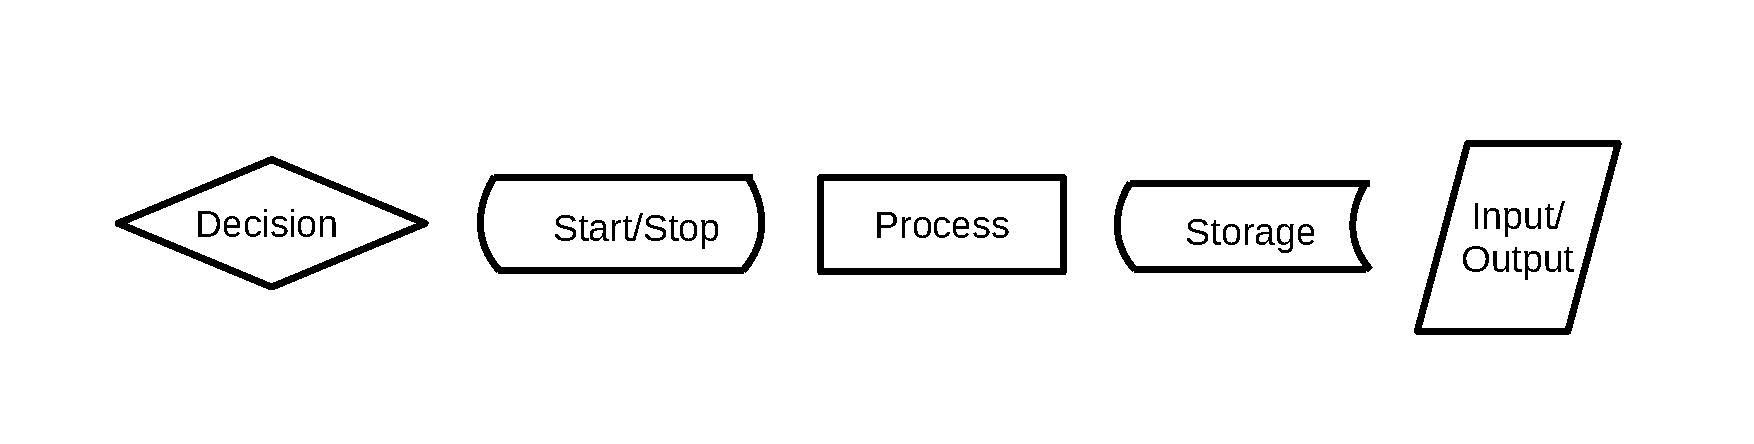
\includegraphics[width=14cm]{FlowchartKey.pdf}\hspace*{\fill}
\end{figure}
\pagebreak

\begin{figure}[H]
\caption{Main Flowchart} \label{fig:LogInFlowchart}
\hfill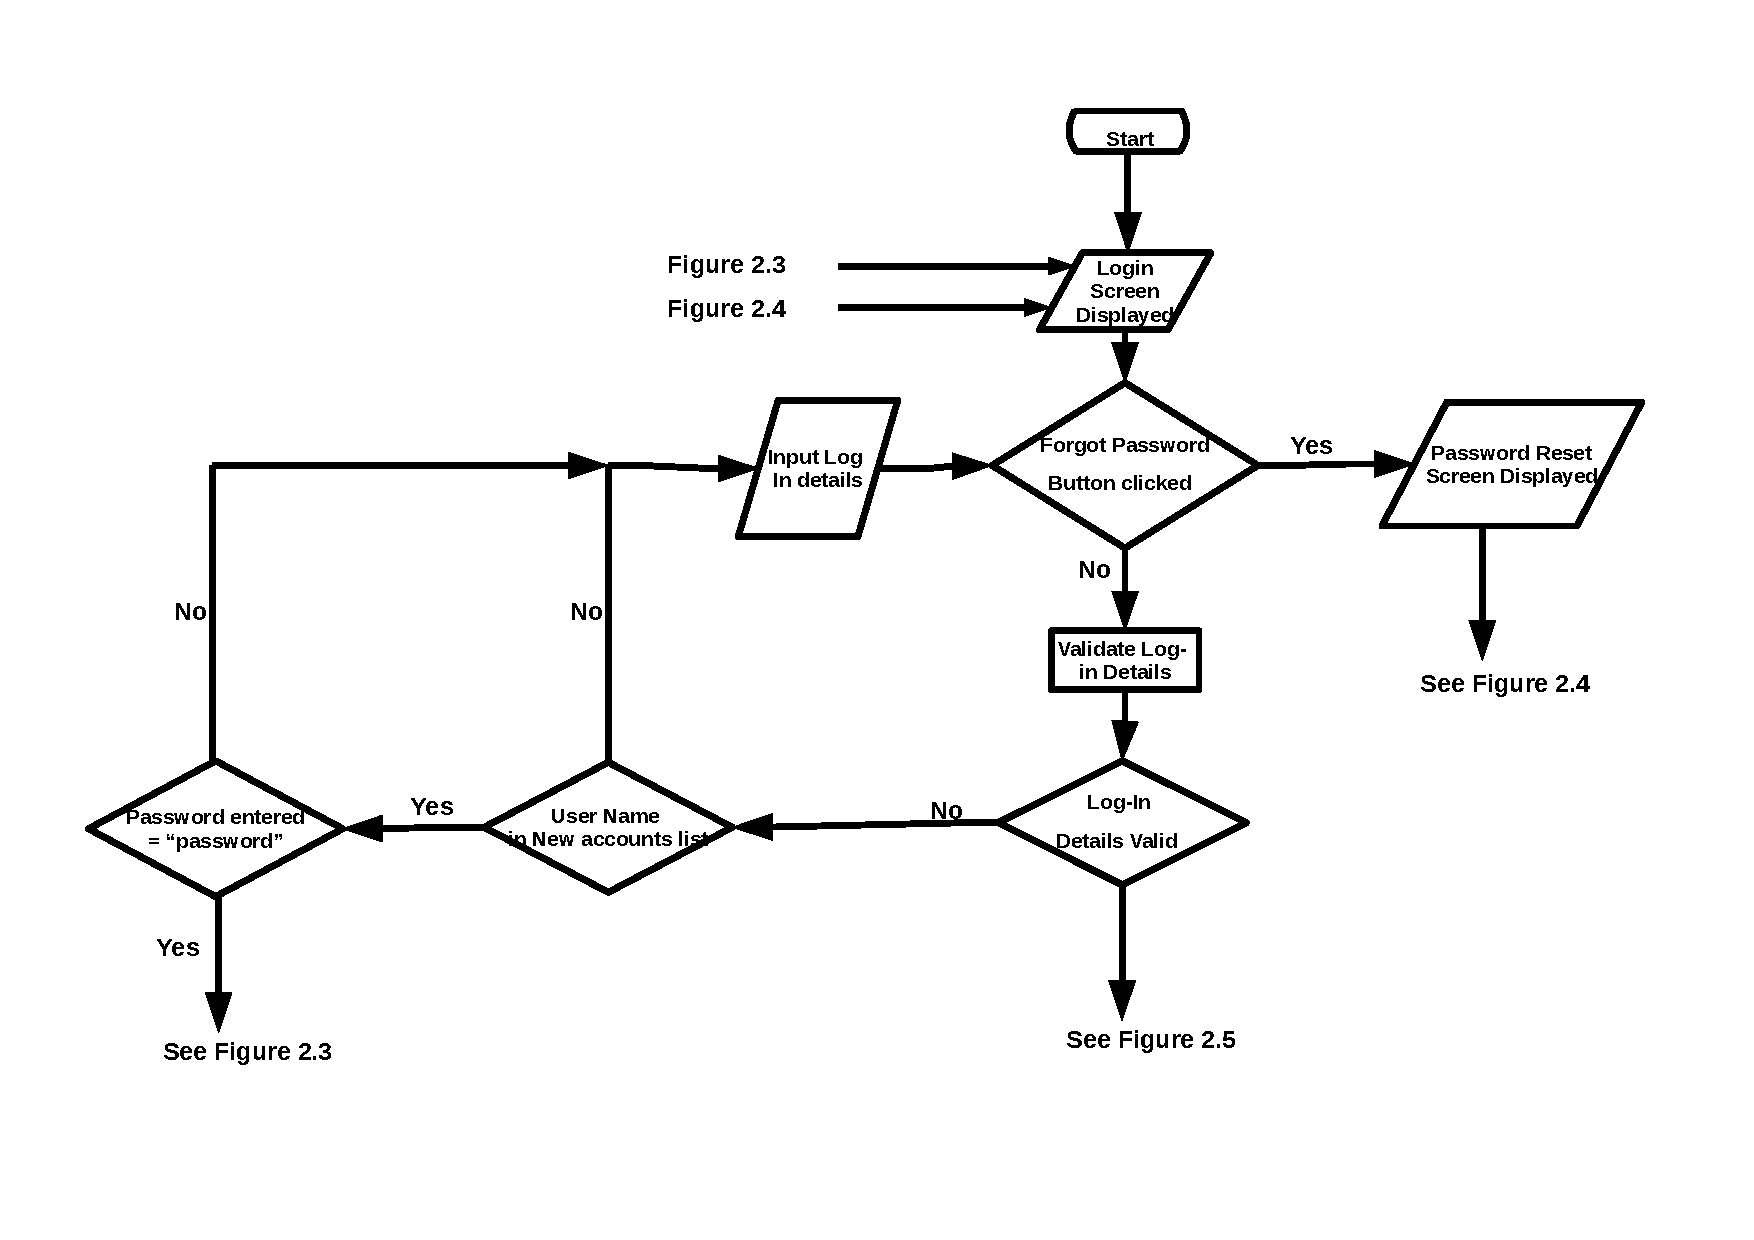
\includegraphics[scale=0.65]{FlowchartMain.pdf}\hspace*{\fill}
\end{figure}
\pagebreak

\begin{figure}[H]
\caption{New Password Flowchart} \label{fig:New Password Flowchart}
\hfill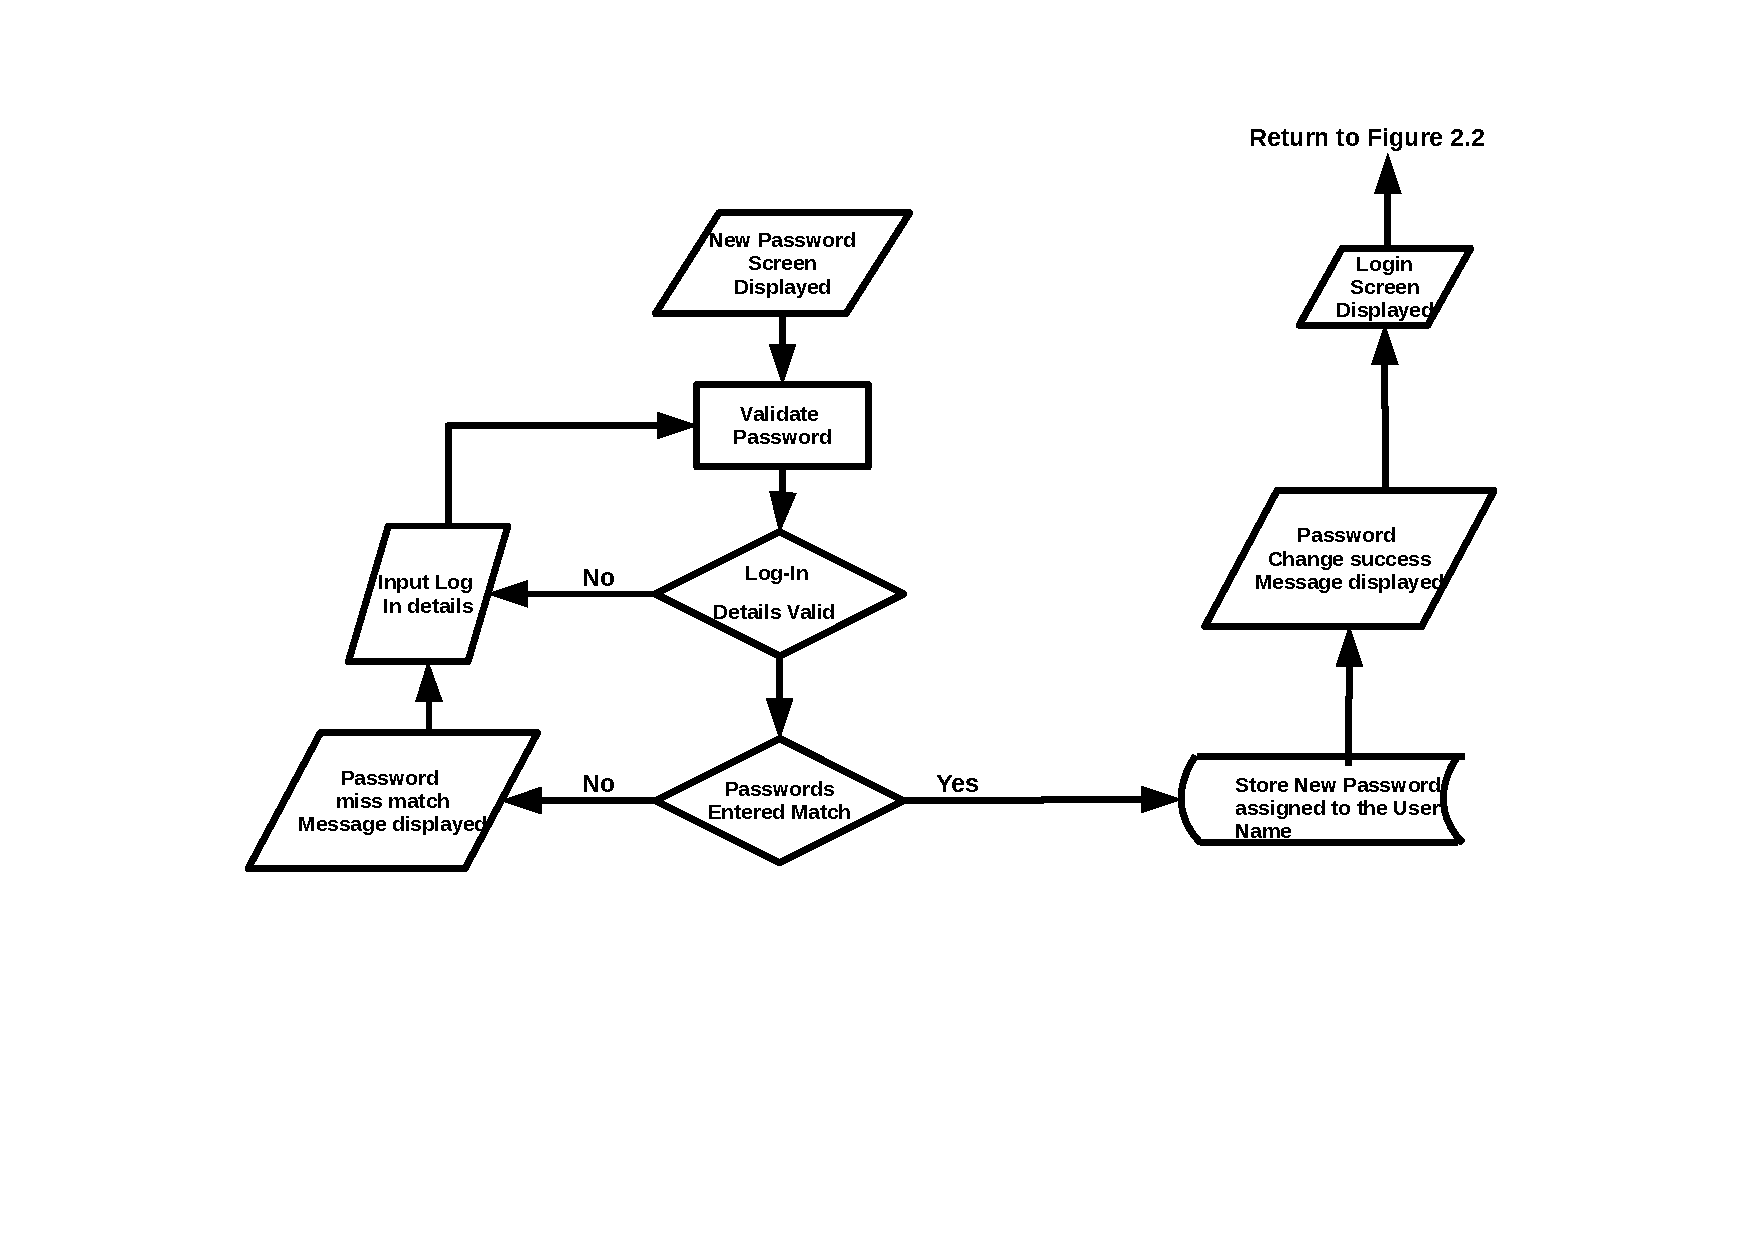
\includegraphics[scale=0.65]{NewPasswordFlowchart.pdf}\hspace*{\fill}
\end{figure}
\pagebreak


\begin{figure}[H]
\caption{Password Reset Flowchart} \label{fig:Password Reset Flowchart}
\hfill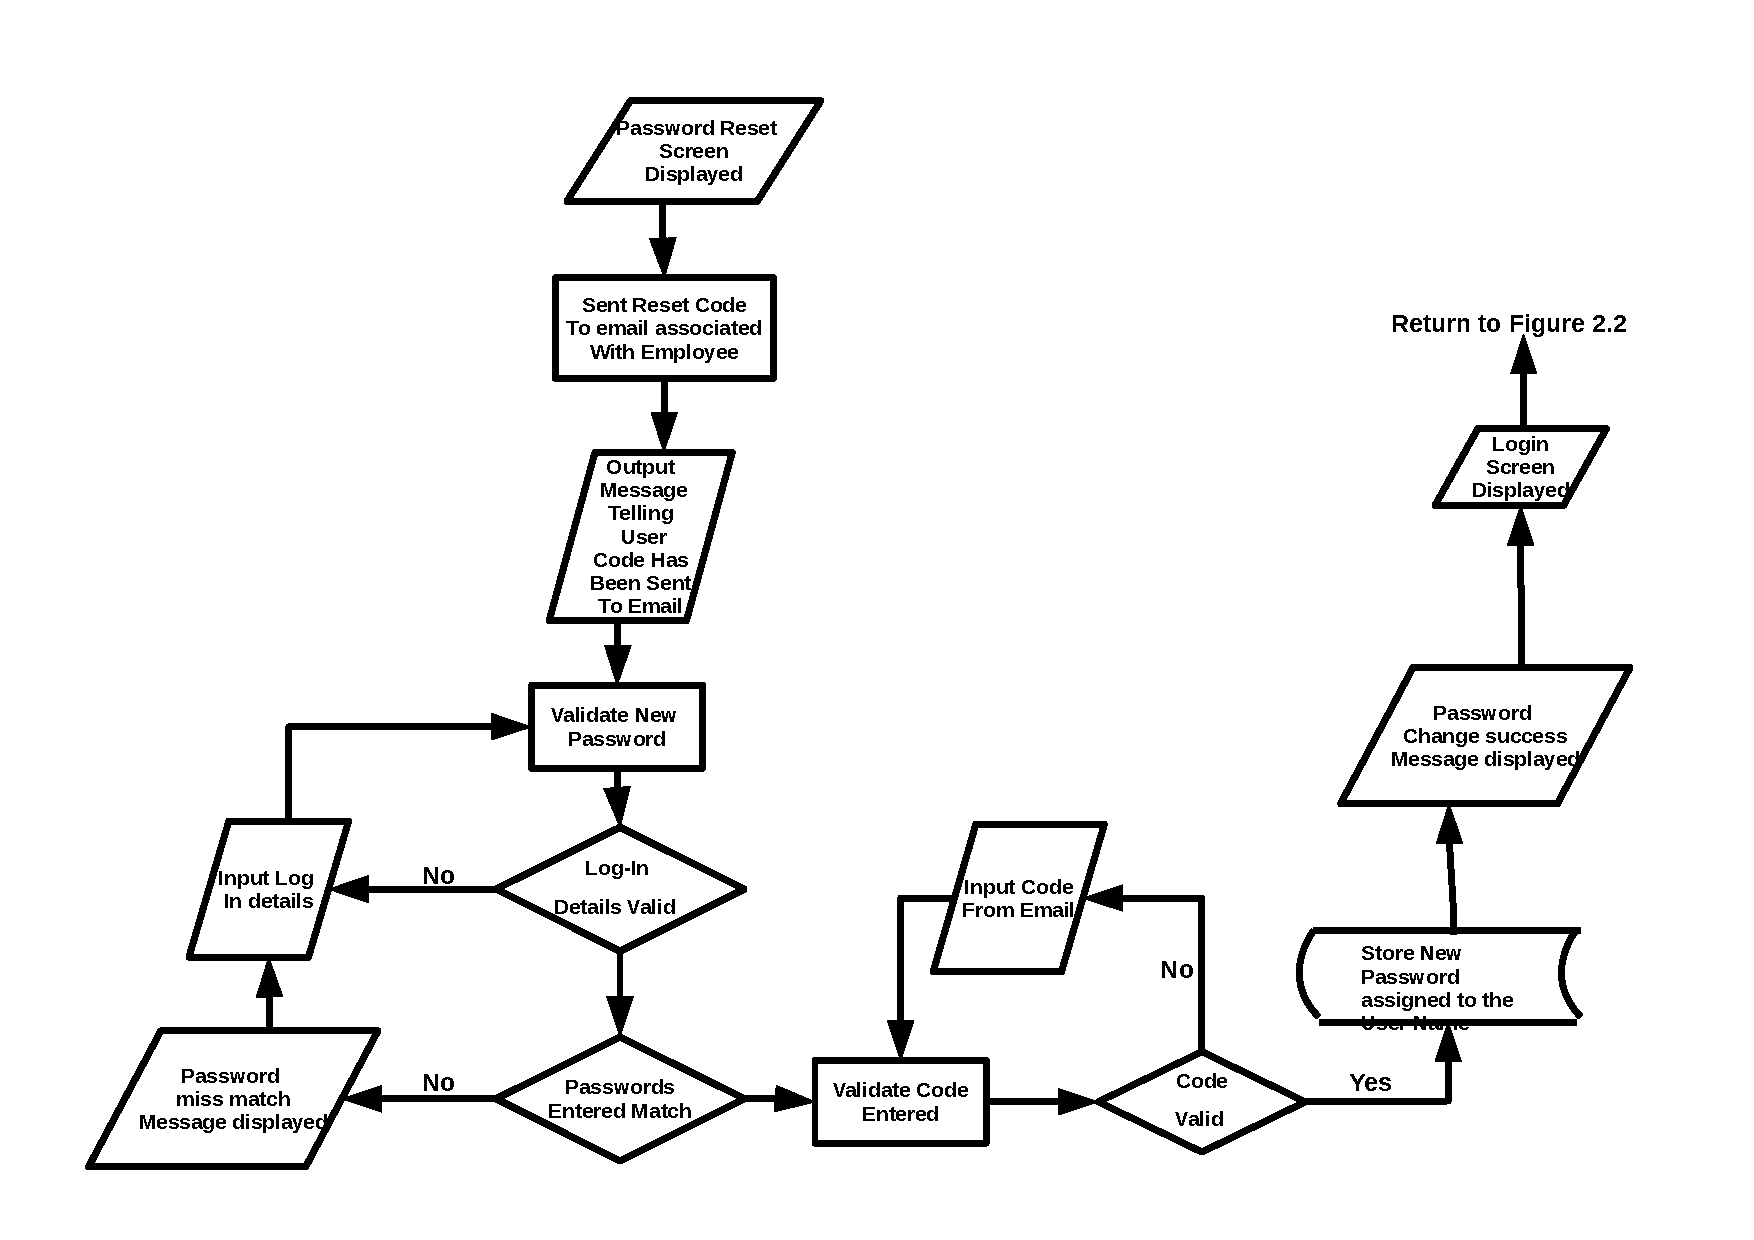
\includegraphics[scale=0.65]{PasswordResetFlowchart.pdf}\hspace*{\fill}
\end{figure}
\pagebreak

\end{landscape}

\begin{figure}[H]
\caption{Options Menu} \label{fig:Options Menu}
\hfill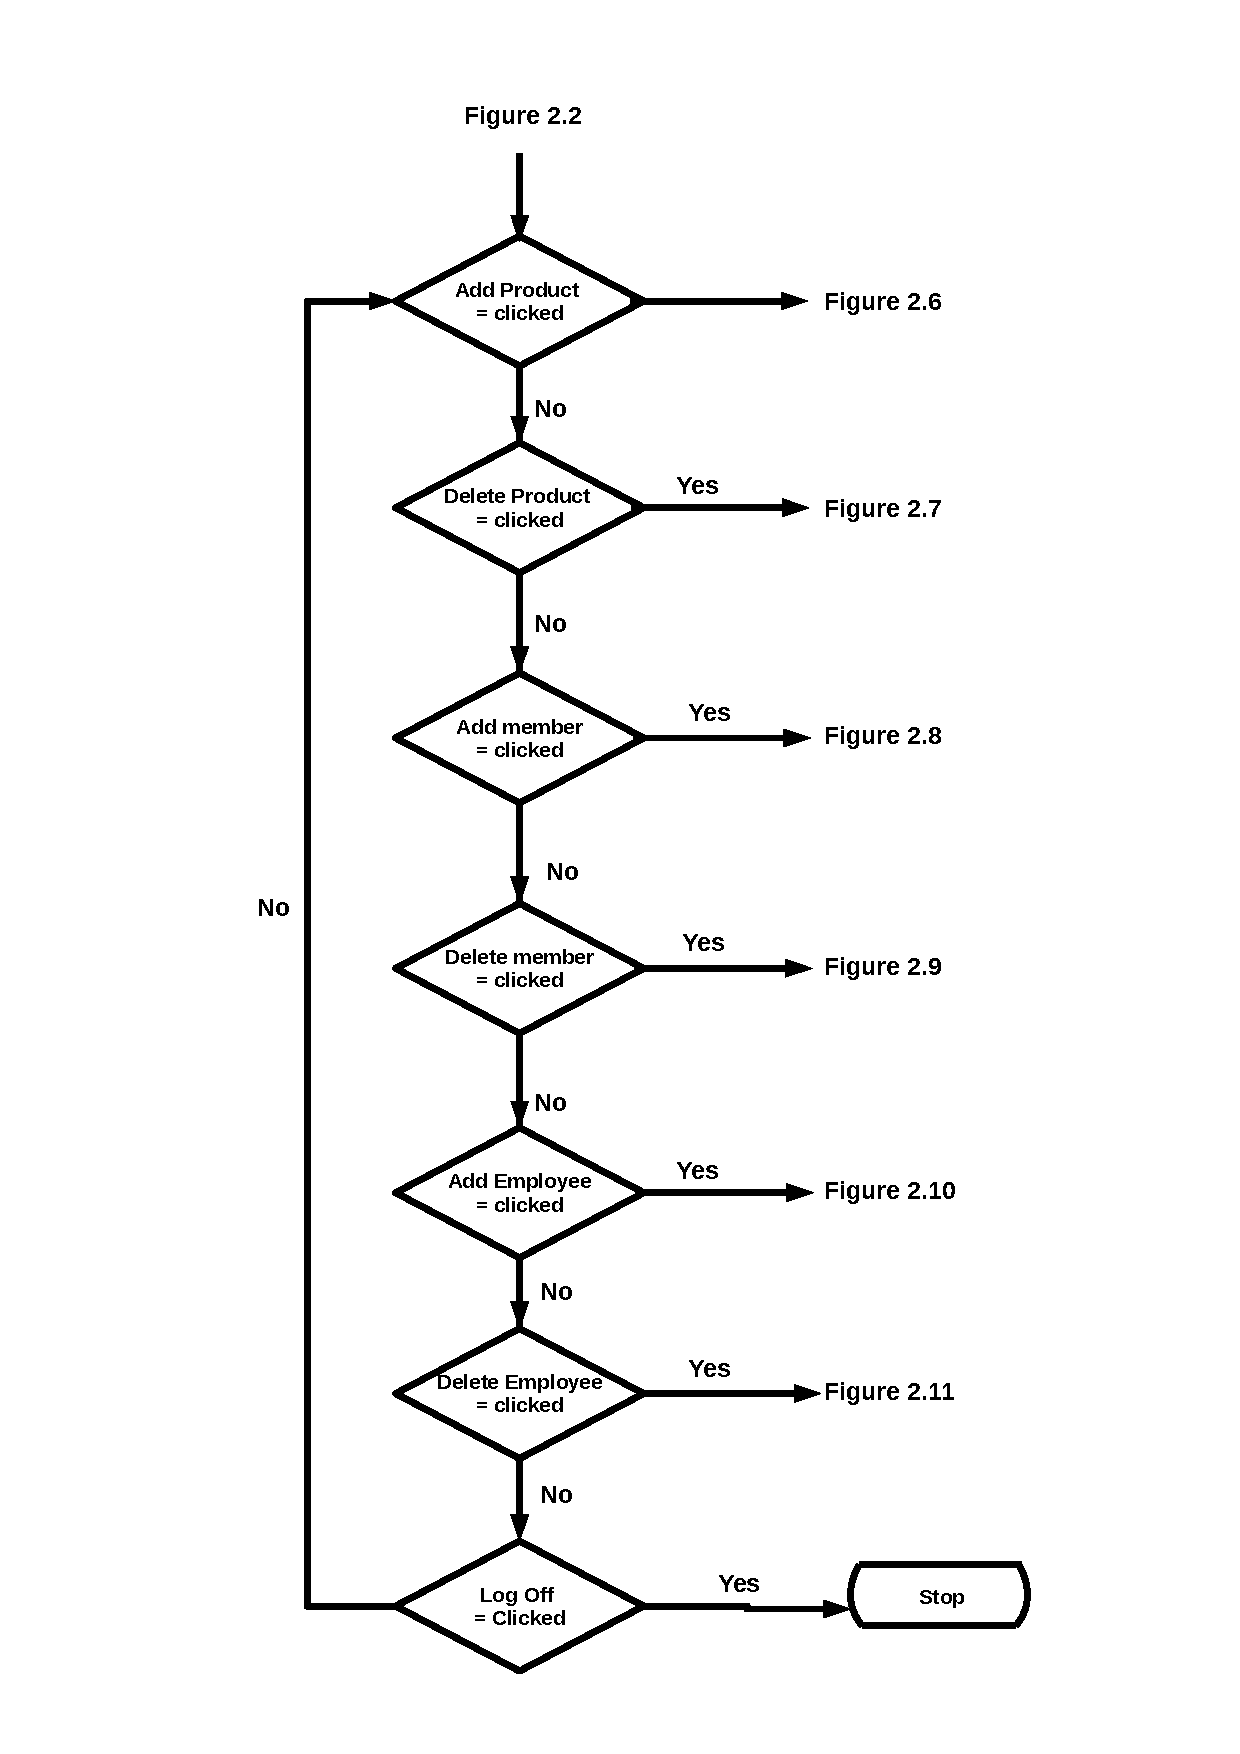
\includegraphics[scale=0.65]{Figure25.pdf}\hspace*{\fill}
\end{figure}
\pagebreak

\begin{landscape}
\begin{figure}[H]
\caption{Add a New Product} \label{fig:Add a New Product}
\hfill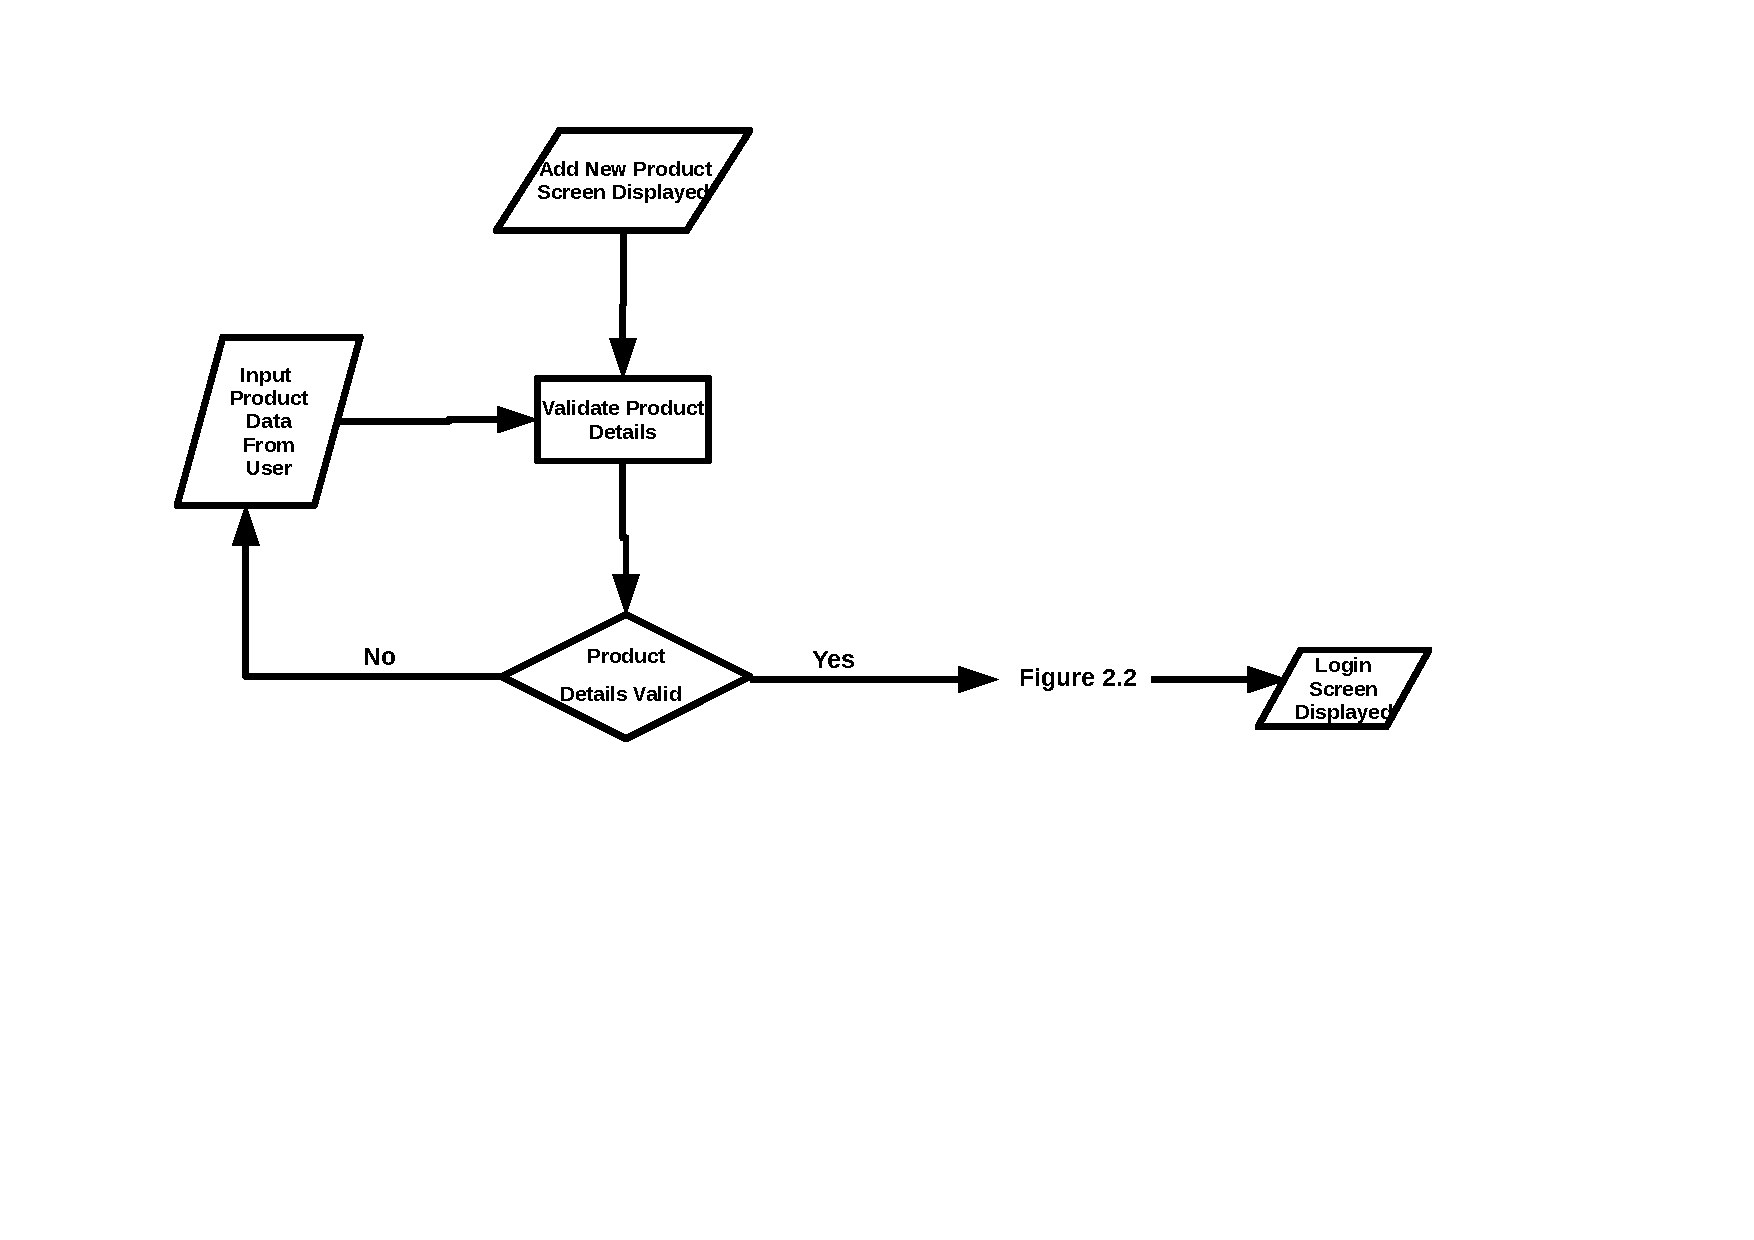
\includegraphics[scale=0.65]{Figure26.pdf}\hspace*{\fill}
\end{figure}
\pagebreak

\begin{figure}[H]
\caption{Delete a Product} \label{fig:Delete a Product}
\hfill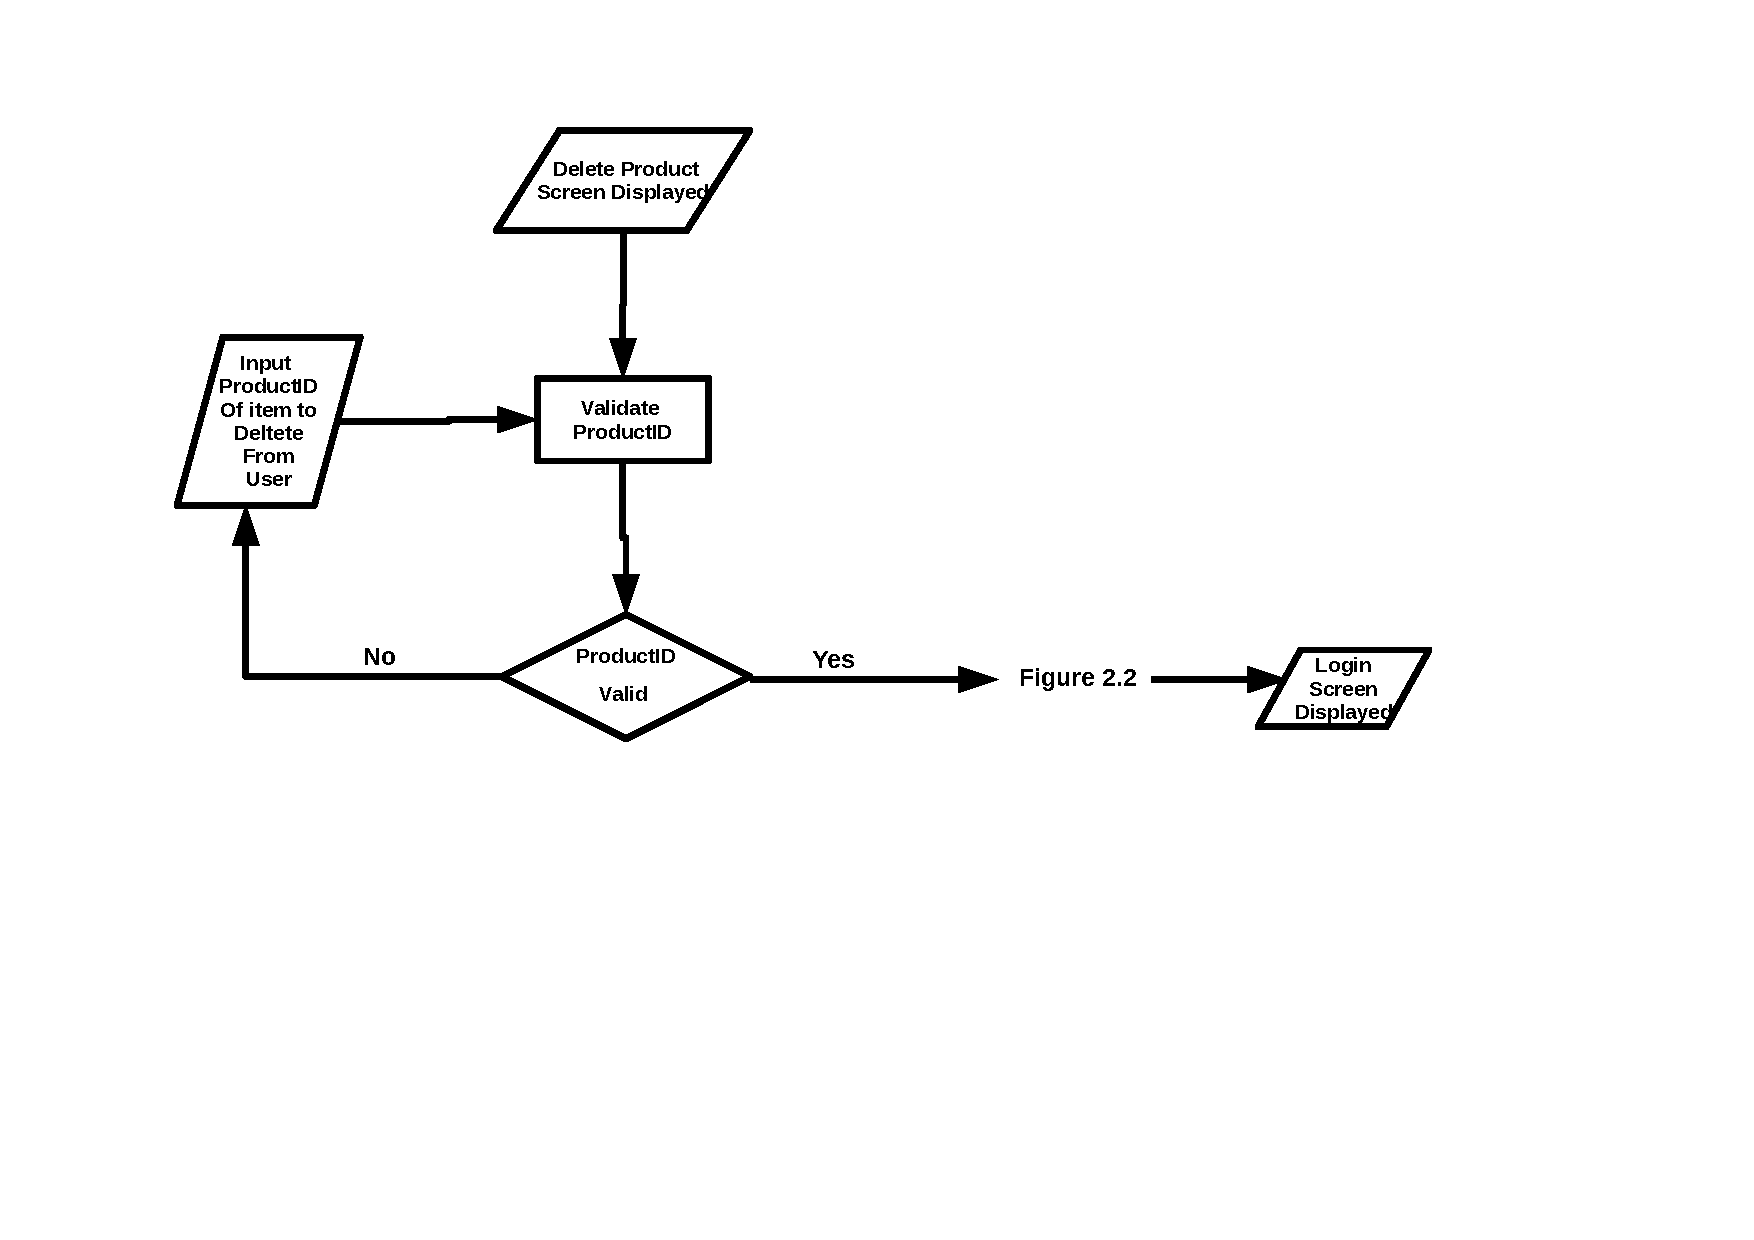
\includegraphics[scale=0.65]{Figure27.pdf}\hspace*{\fill}
\end{figure}
\pagebreak

\begin{figure}[H]
\caption{Add a Member} \label{fig:Add a Member}
\hfill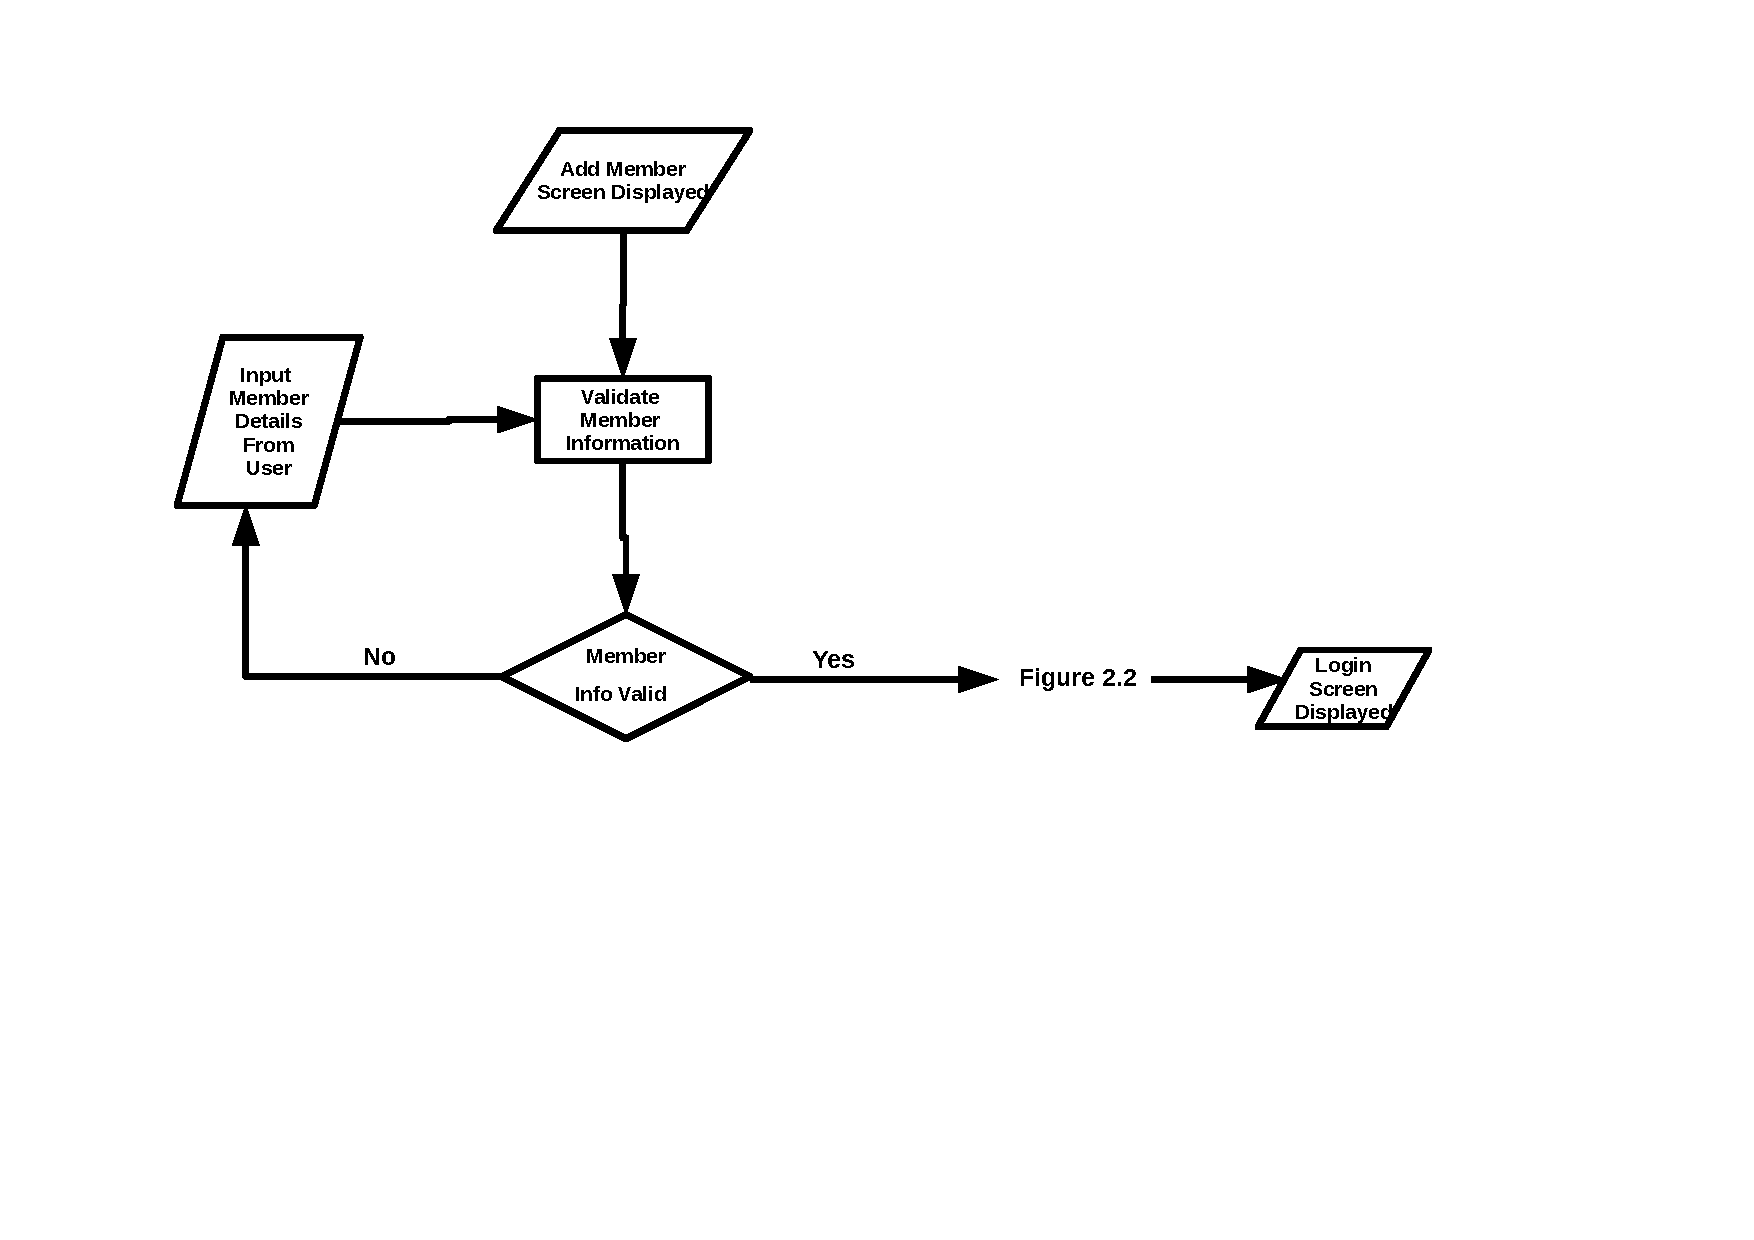
\includegraphics[scale=0.65]{Figure28.pdf}\hspace*{\fill}
\end{figure}
\pagebreak

\begin{figure}[H]
\caption{Delete a Member} \label{fig:Delete a Member}
\hfill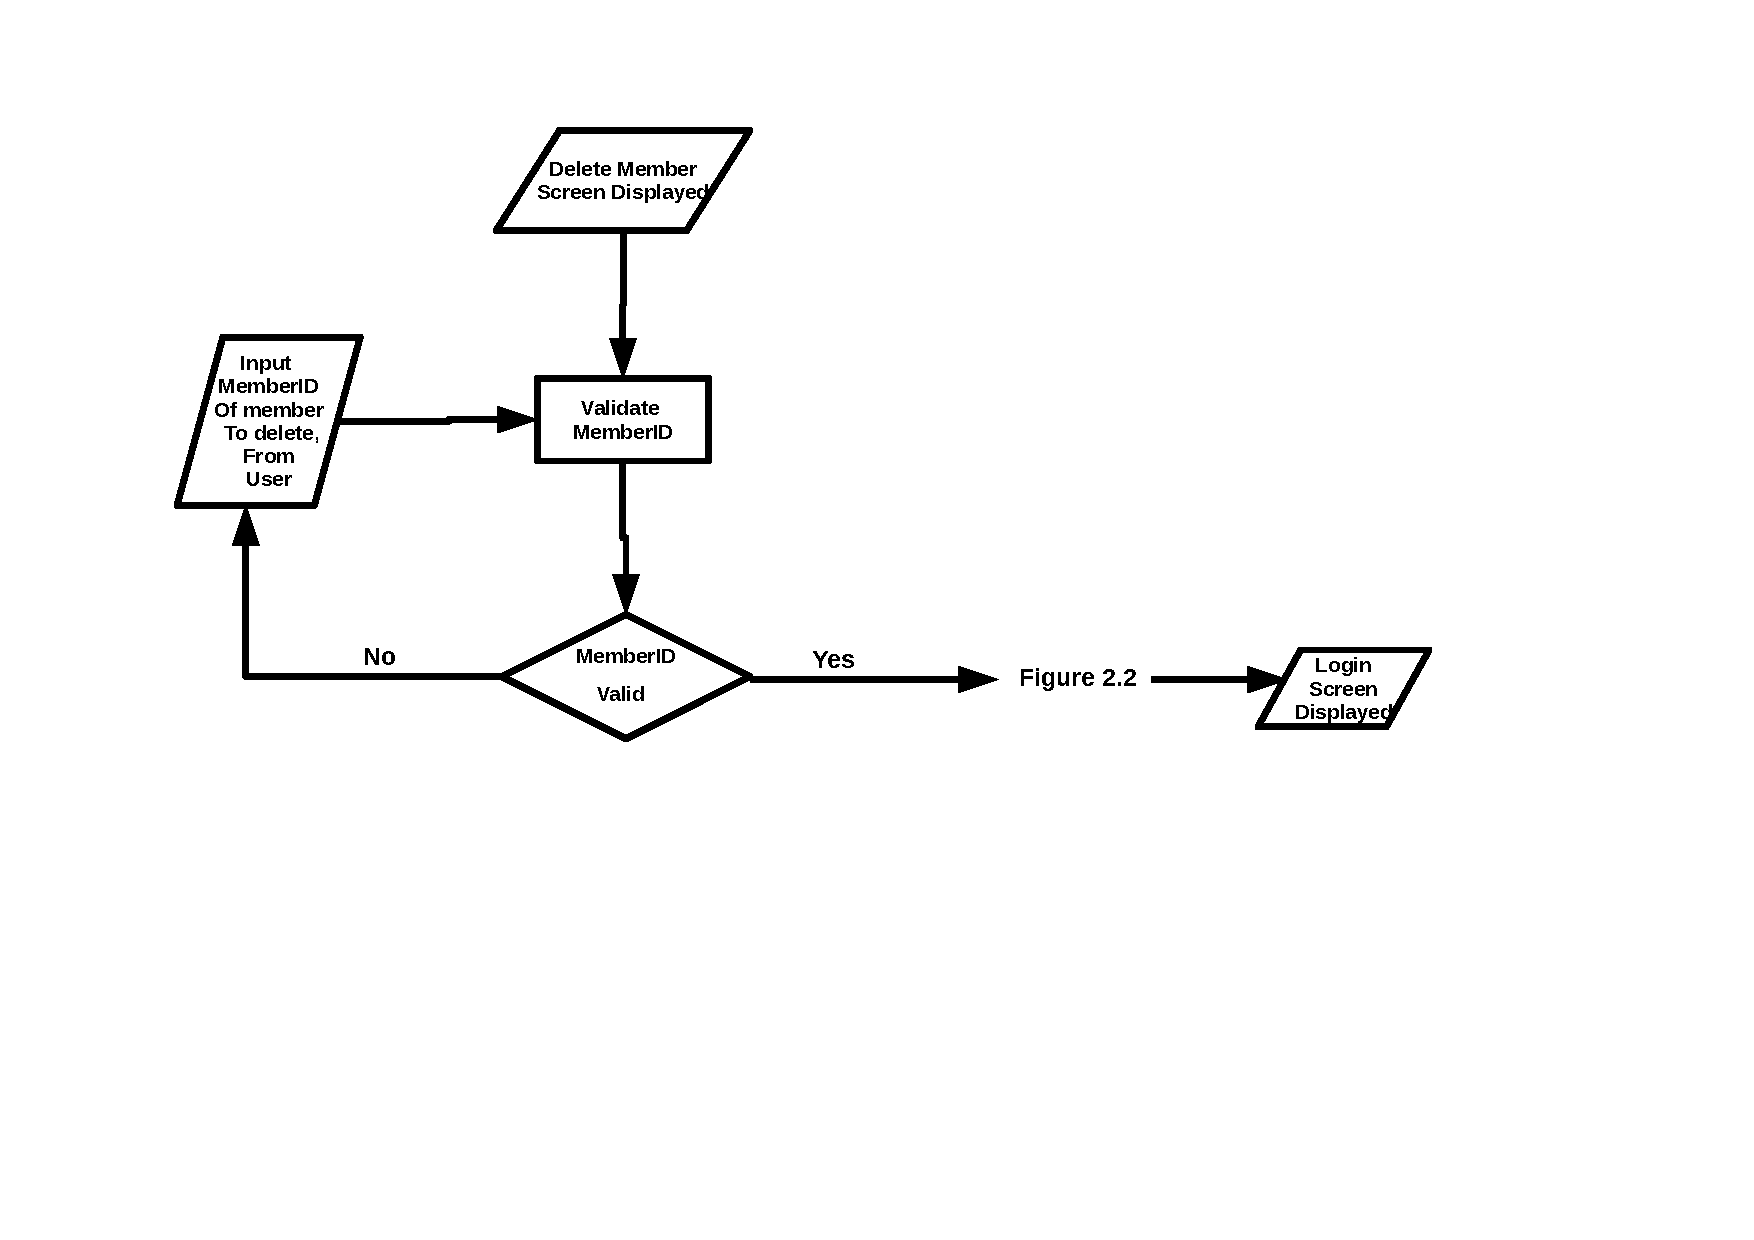
\includegraphics[scale=0.65]{Figure29.pdf}\hspace*{\fill}
\end{figure}
\pagebreak

\begin{figure}[H]
\caption{Add an Employee} \label{fig:Add an Employee}
\hfill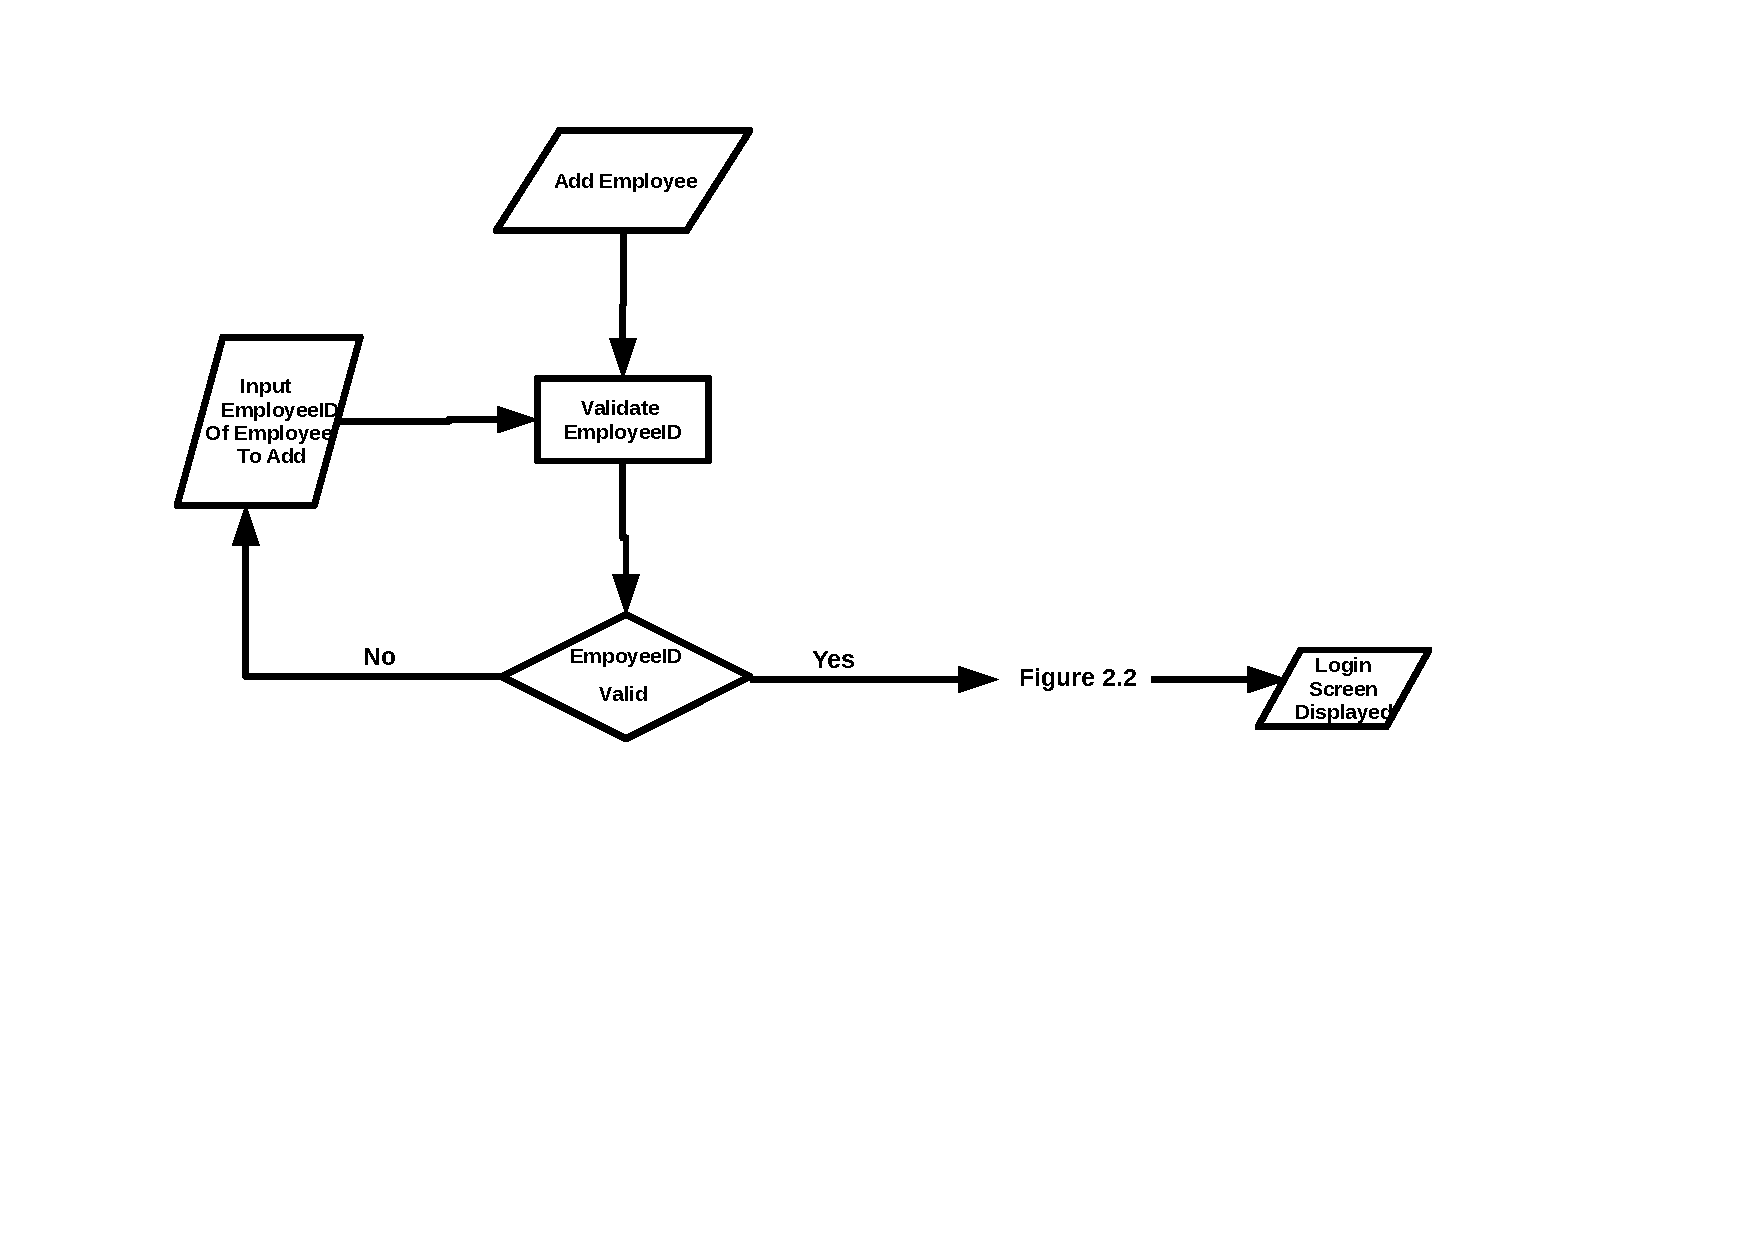
\includegraphics[scale=0.65]{Figure31.pdf}\hspace*{\fill}
\end{figure}
\pagebreak

\begin{figure}[H]
\caption{Delete an Employee} \label{fig:Delete an Employee}
\hfill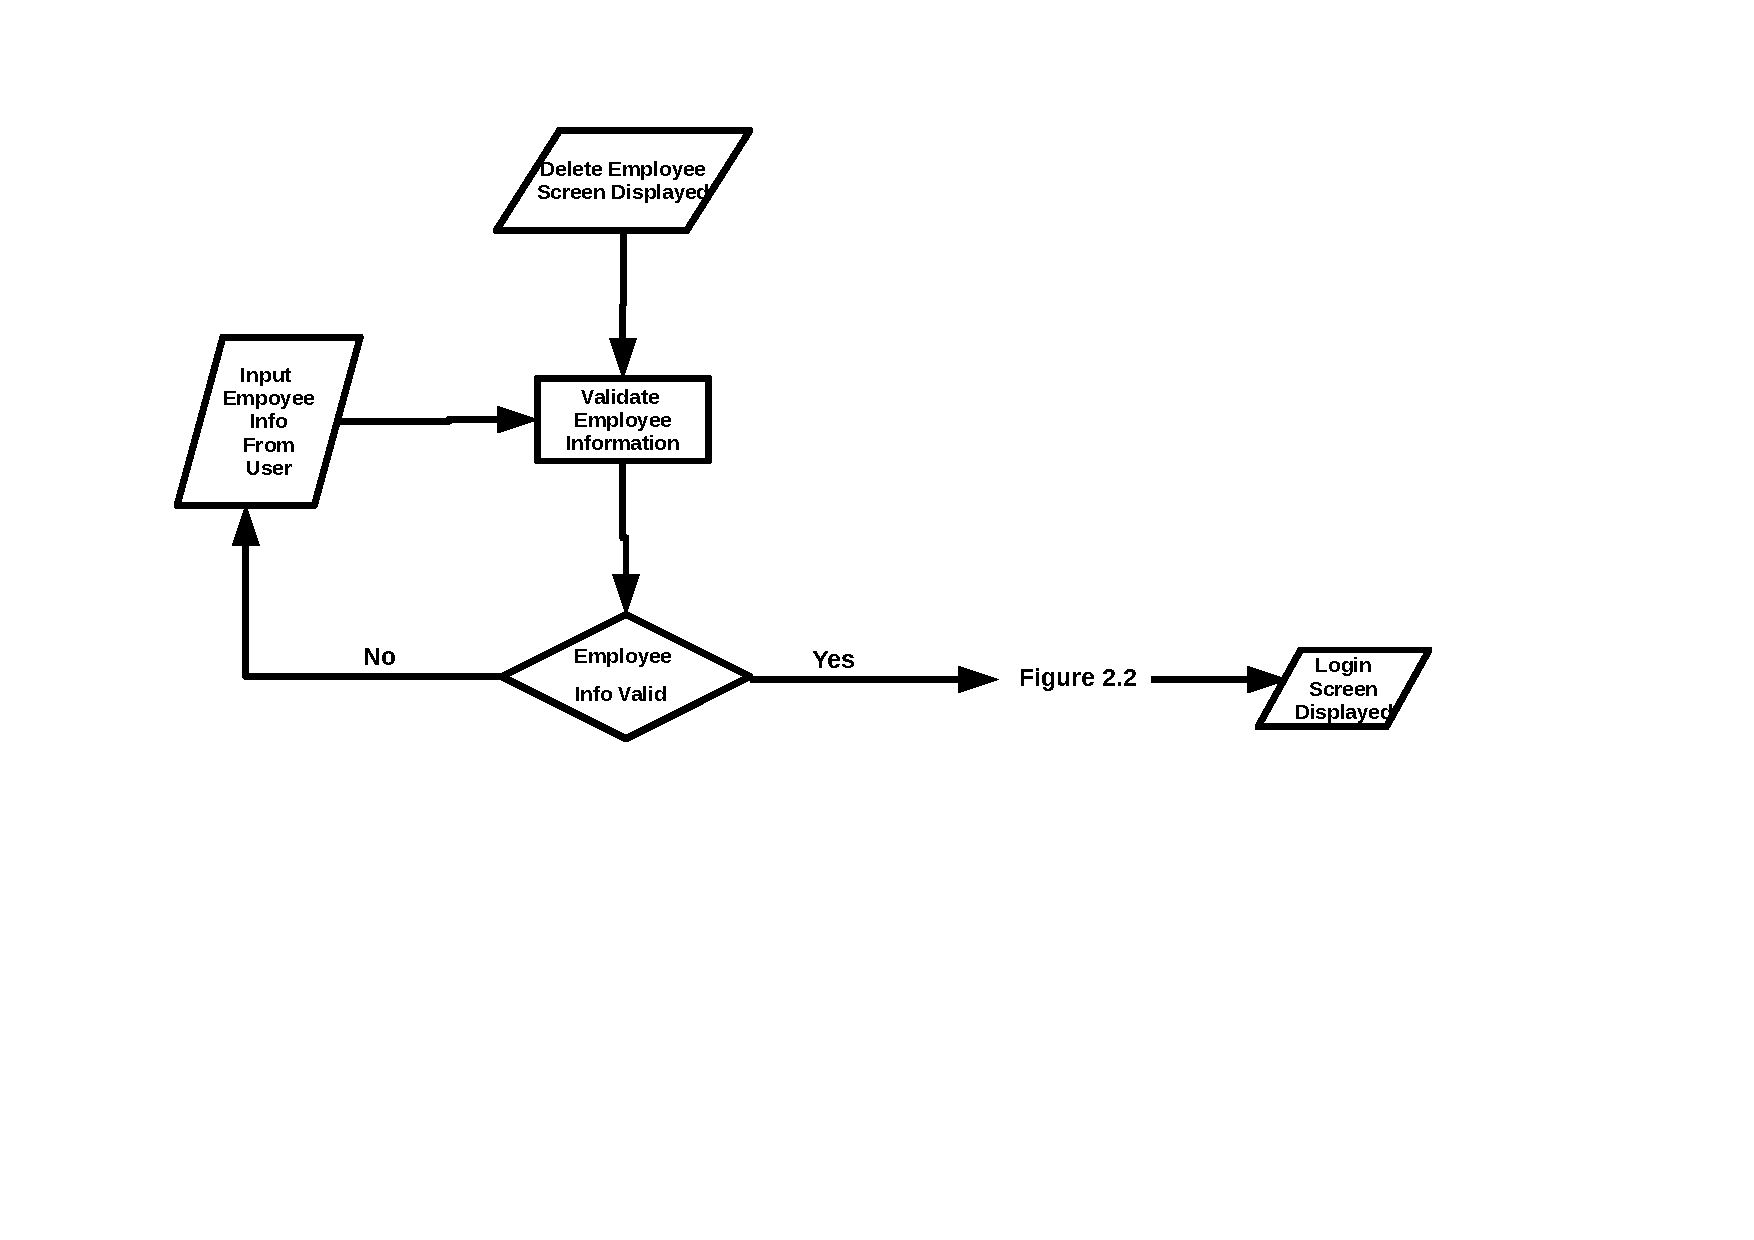
\includegraphics[scale=0.65]{Figure30.pdf}\hspace*{\fill}
\end{figure}
\pagebreak

\end{landscape}
\section{User Interface Designs}


\begin{figure}[H]
\caption{Log In Interface} \label{fig: Log In Interface}
\hfill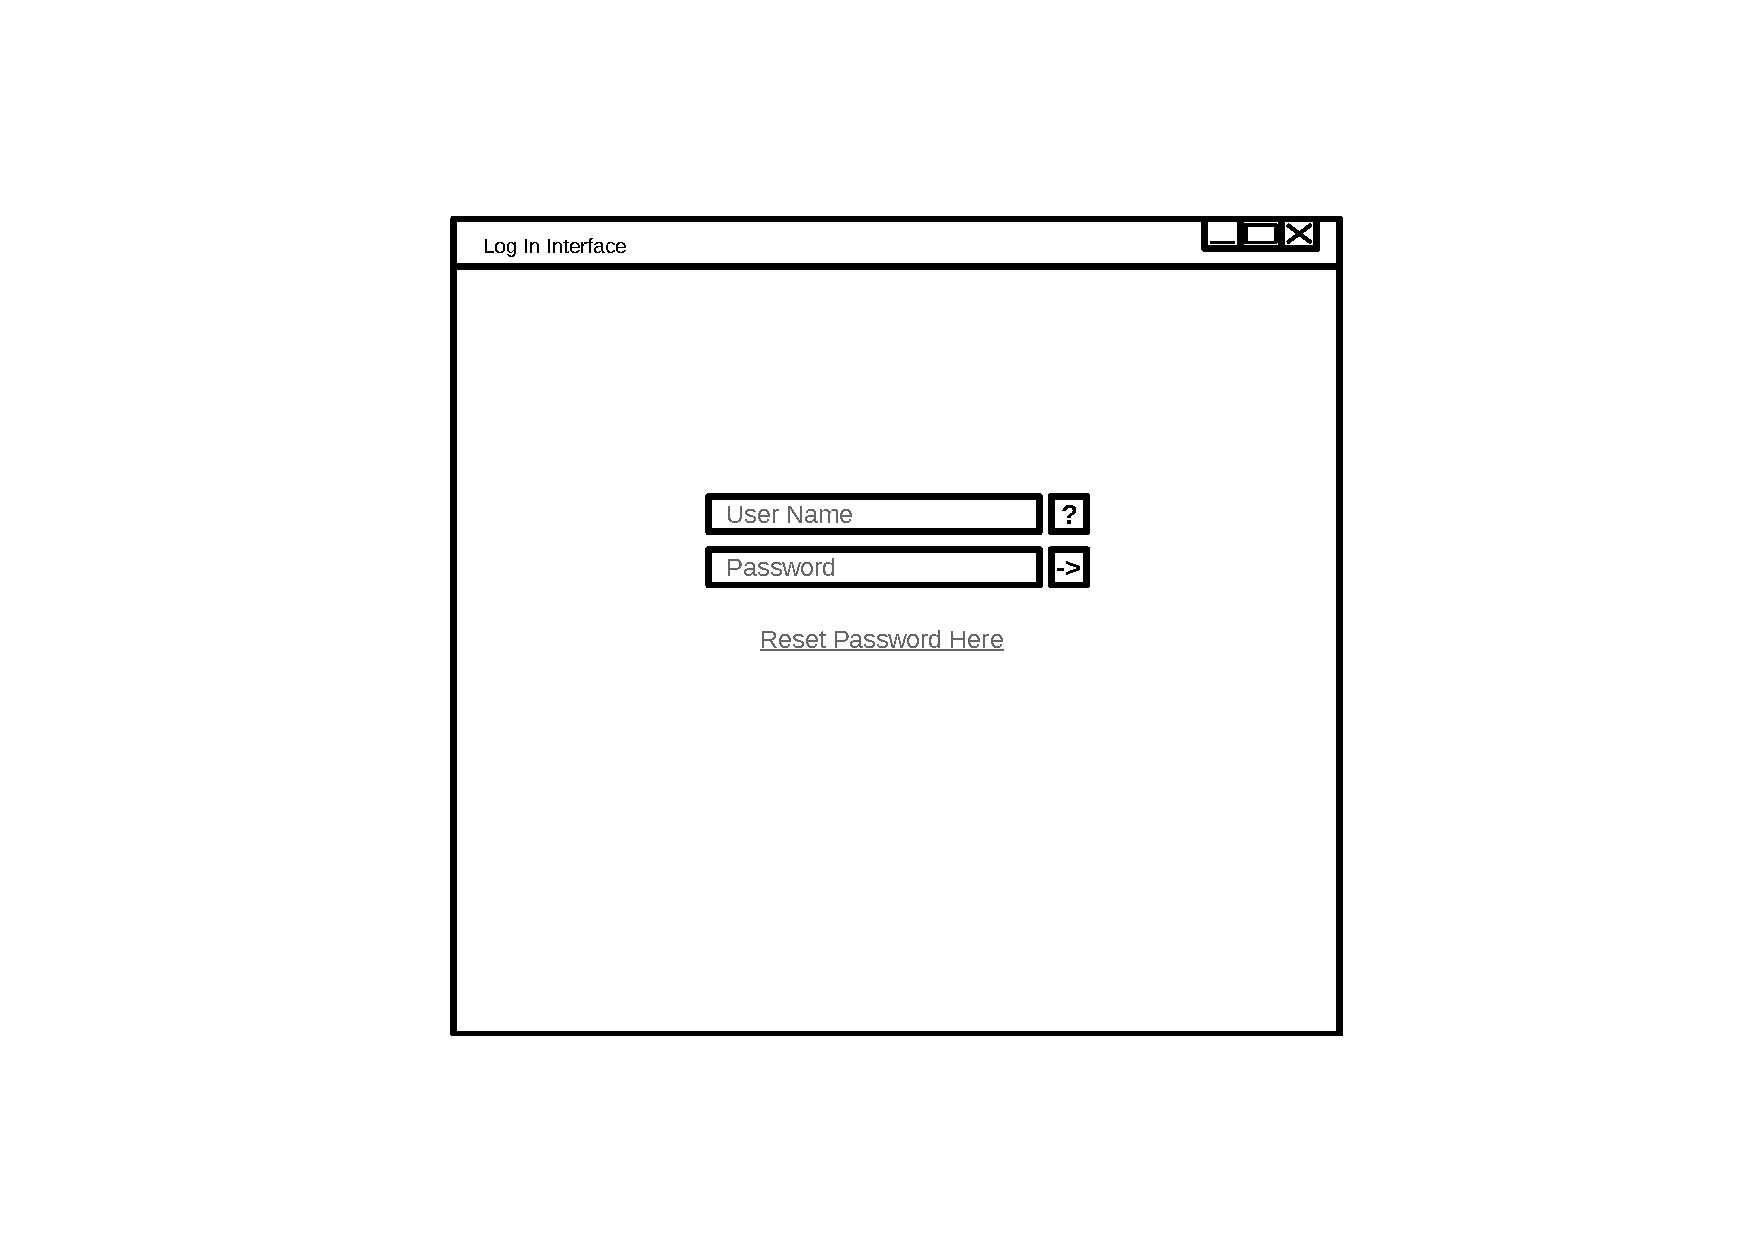
\includegraphics[width = 14cm]{Log-InInterfaceDiagramEdited.pdf}\hspace*{\fill}
\end{figure}


\begin{flushleft}
Looking at Figure 2.12 on Page 51, You can see the Employee Log in interface. The Log In interface contains two fields in which the username and password can be entered and two push buttons, one being the `?' and the other being `->'. The `?' symbol, when clicked, reminds the employee how their username is formed. (First Letter of First Name + Last Name + EmployeeID i.e: MLing03). None of the system is accessible on the log in screen which means that the user MUST log in before they can use the system. This is a security feature as it prevents anyone that does not have a username and password from using the system. The `->' button is simply a click button that checks the employees username and password to see if they are valid. A keyboard shortcut that is commonly assigned to this is `Enter'. \par

If the user clicks on `Reset Password Here' Then the user is directed to a page where they enter a new password to use. A secuirty measure to stop the password being changed by anyone is that the system sends an email to the address assigned to that account, that way, only the employee in which the account is associated with can change the password.  Once the user has logged in, the menu bar should be displayed which will allow the user to navigate between the interfaces.\par

\end{flushleft}

\begin{figure}[H]
\caption{Product Search Interface} \label{fig: Product Search Interface}
\hfill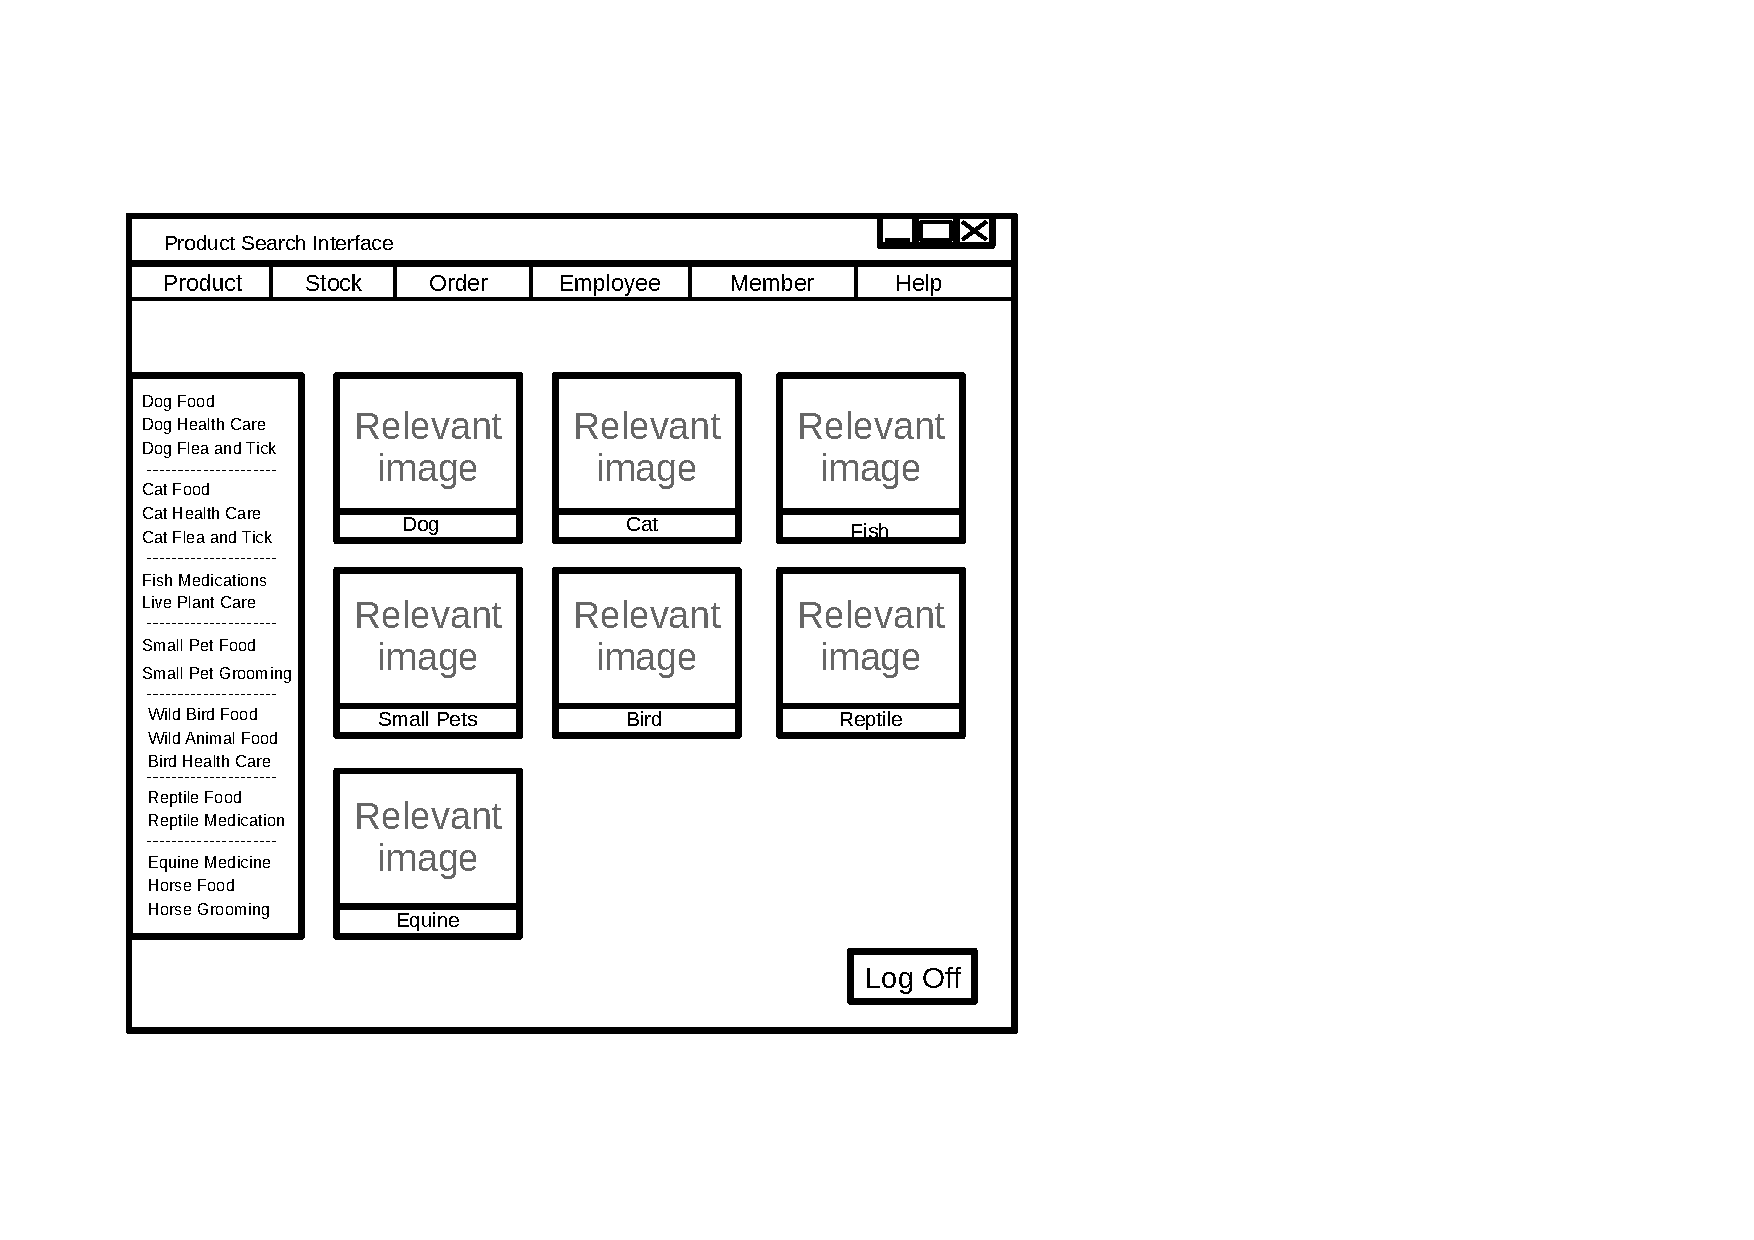
\includegraphics[width = 14cm]{UIDProductSeachInterfaceEdited.pdf}\hspace*{\fill}
\end{figure}

Figure 2.13 is the Product Search Interface, This will also act as the main menu as this will be the most commonly used interface. Once the user has logged in, The six tabs are always displayed at the top of the application, no matter what interface they are on (other than the log in interface). \par

The product Search interface is used when the user wants to find a specific product. This can be done one of three ways. If the user knows the name of the product they are looking for, they can simply use the search bar which is described later in the User Interface Design Section. Alternatively the user can Go to the Product Search interface and click on the large buttons that are made up of an Animal and a picture of that animal, by clicking on that button, The user will then have to click on the category in which the product falls under(i.e food / health care) The user will then be given a table of all the products that fall under that category. The user will be able to sort the products to find the product they are looking for. \par

However, going from a product from one category to a product from another category may be quite confusing going back and forth between categories, pressing multiple buttons. Therefore a list down the left hand side of the page has Each Category Sorted into each Animal. The user can then jsut simply click on the category and they will be taken straight to the products. This method will allow the user to find products faster by reducing time selecting categories. \par

When The user has finished using the system, they can return to the Product Search interface and click the `Log Off' button under the Options Tab in the MenuBar. This will log the user out and will require an employee to enter their log in details before the system can be accessed again. if the application is closed using the close button in the top right hand corner, without the user logging out, the user will automatically be logged out. However if the user clicks the close button, a warning message will be displayed to confirm they want to close the application. This prevents the application from closing when the user accidentally clicks the close button. \par

\begin{figure}[H]
\caption{Right Click Options For MenuBars} \label{fig:Right Click Options For MenuBars}
\hfill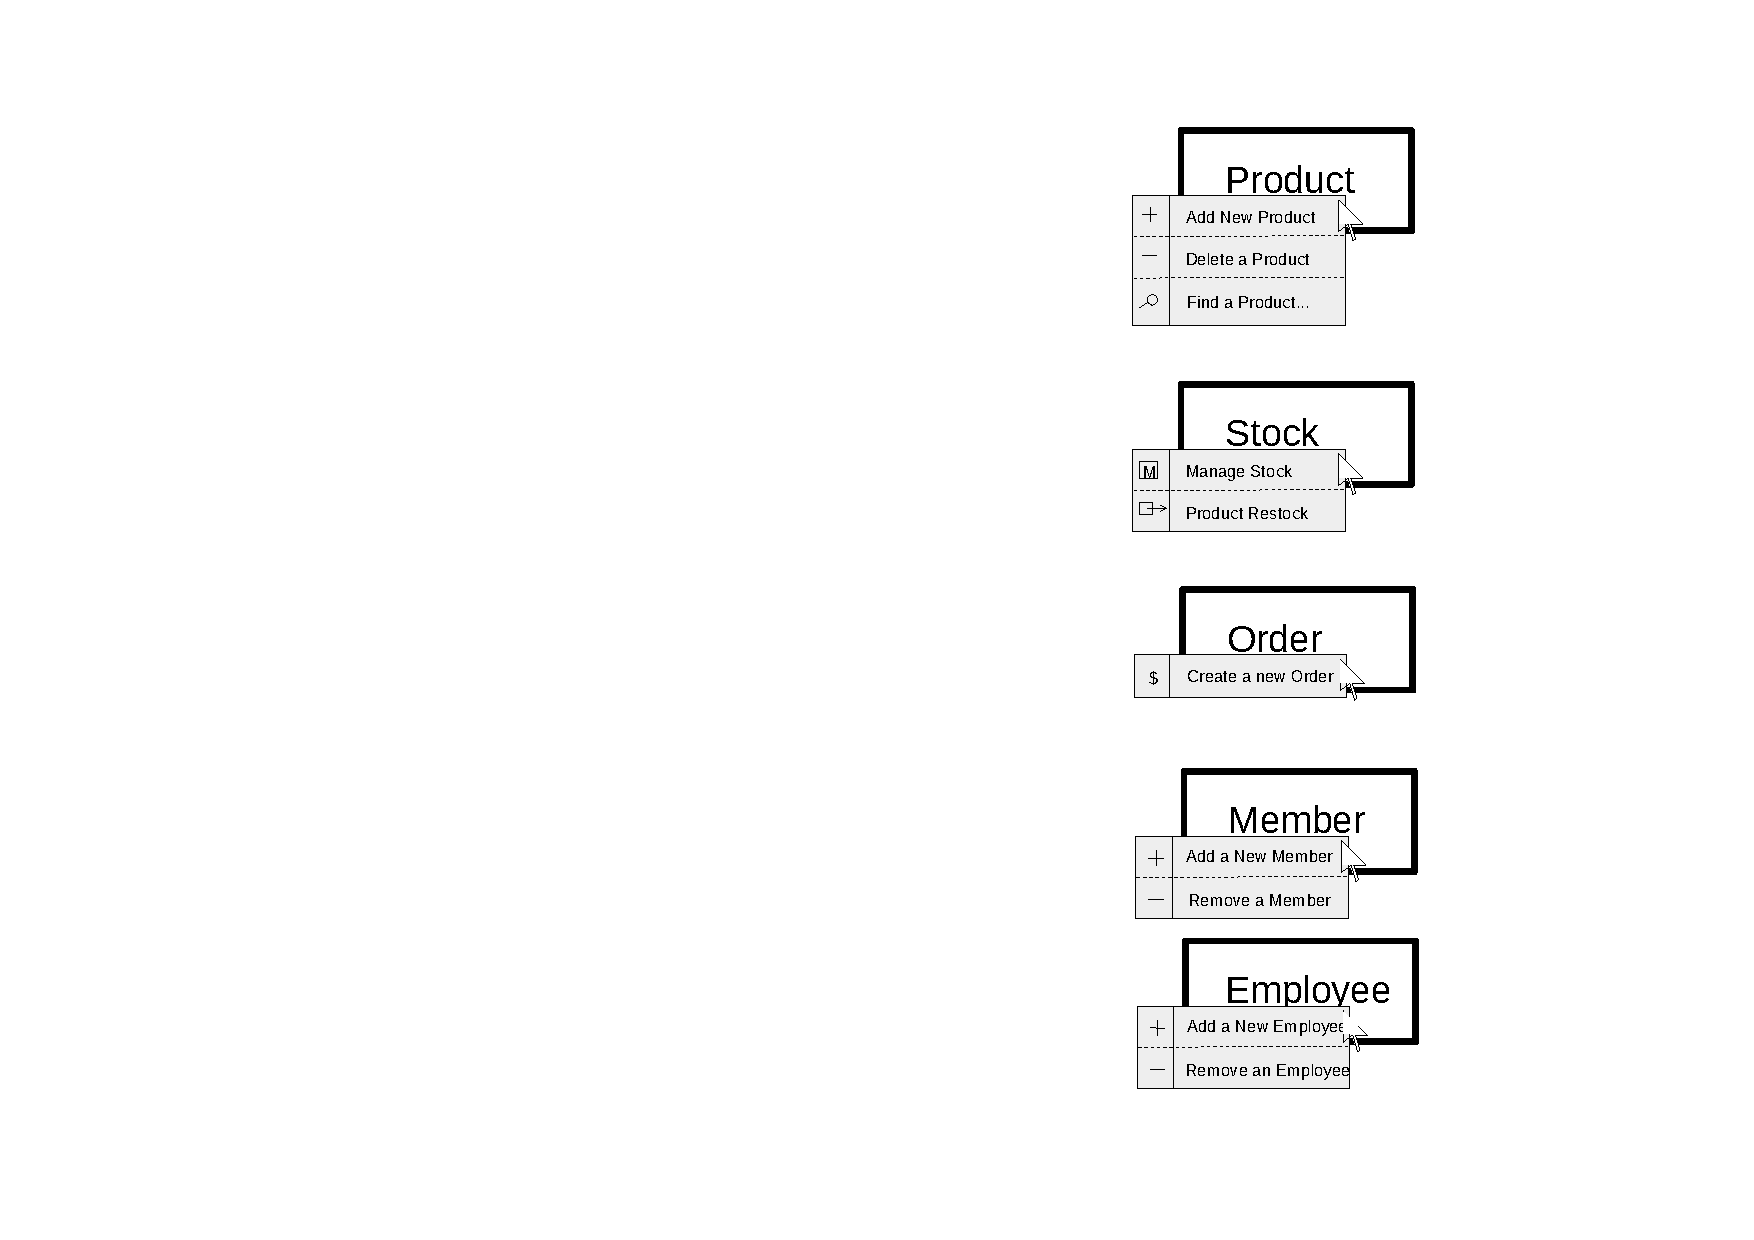
\includegraphics[width = 6cm]{UIDProductSeachInterfaceMenus.pdf}\hspace*{\fill}
\end{figure}

Looking at Figure 2.14 and referring back to Figure 2.13, we can see the options that appear when each tab is clicked. Each option has a symbol next to it to easily identify the option the user wants. When add new product is selected, the user is taken to the add new product interface. Deleting a Product / Member / Employee Account will ask for the ID for the item they user wants to delete, then remove all the data relating to the ID from the sytem. The Manage Stock, Add New Member and Add new Employee buttons will take the user to the corresponding interface. To navigate between the pages, the user will use the menu to select the page they want to go to. For example, if the user is on the Add new Product screen and wants to go to the Add new Member, They go to the Member Menu then select Add new Member. Their current page will then change to the new page they selected. An example of this is shown below:\par

\begin{figure}[H]
\caption{Right Click Options For MenuBars} \label{fig:Right Click Options For MenuBars}
\hfill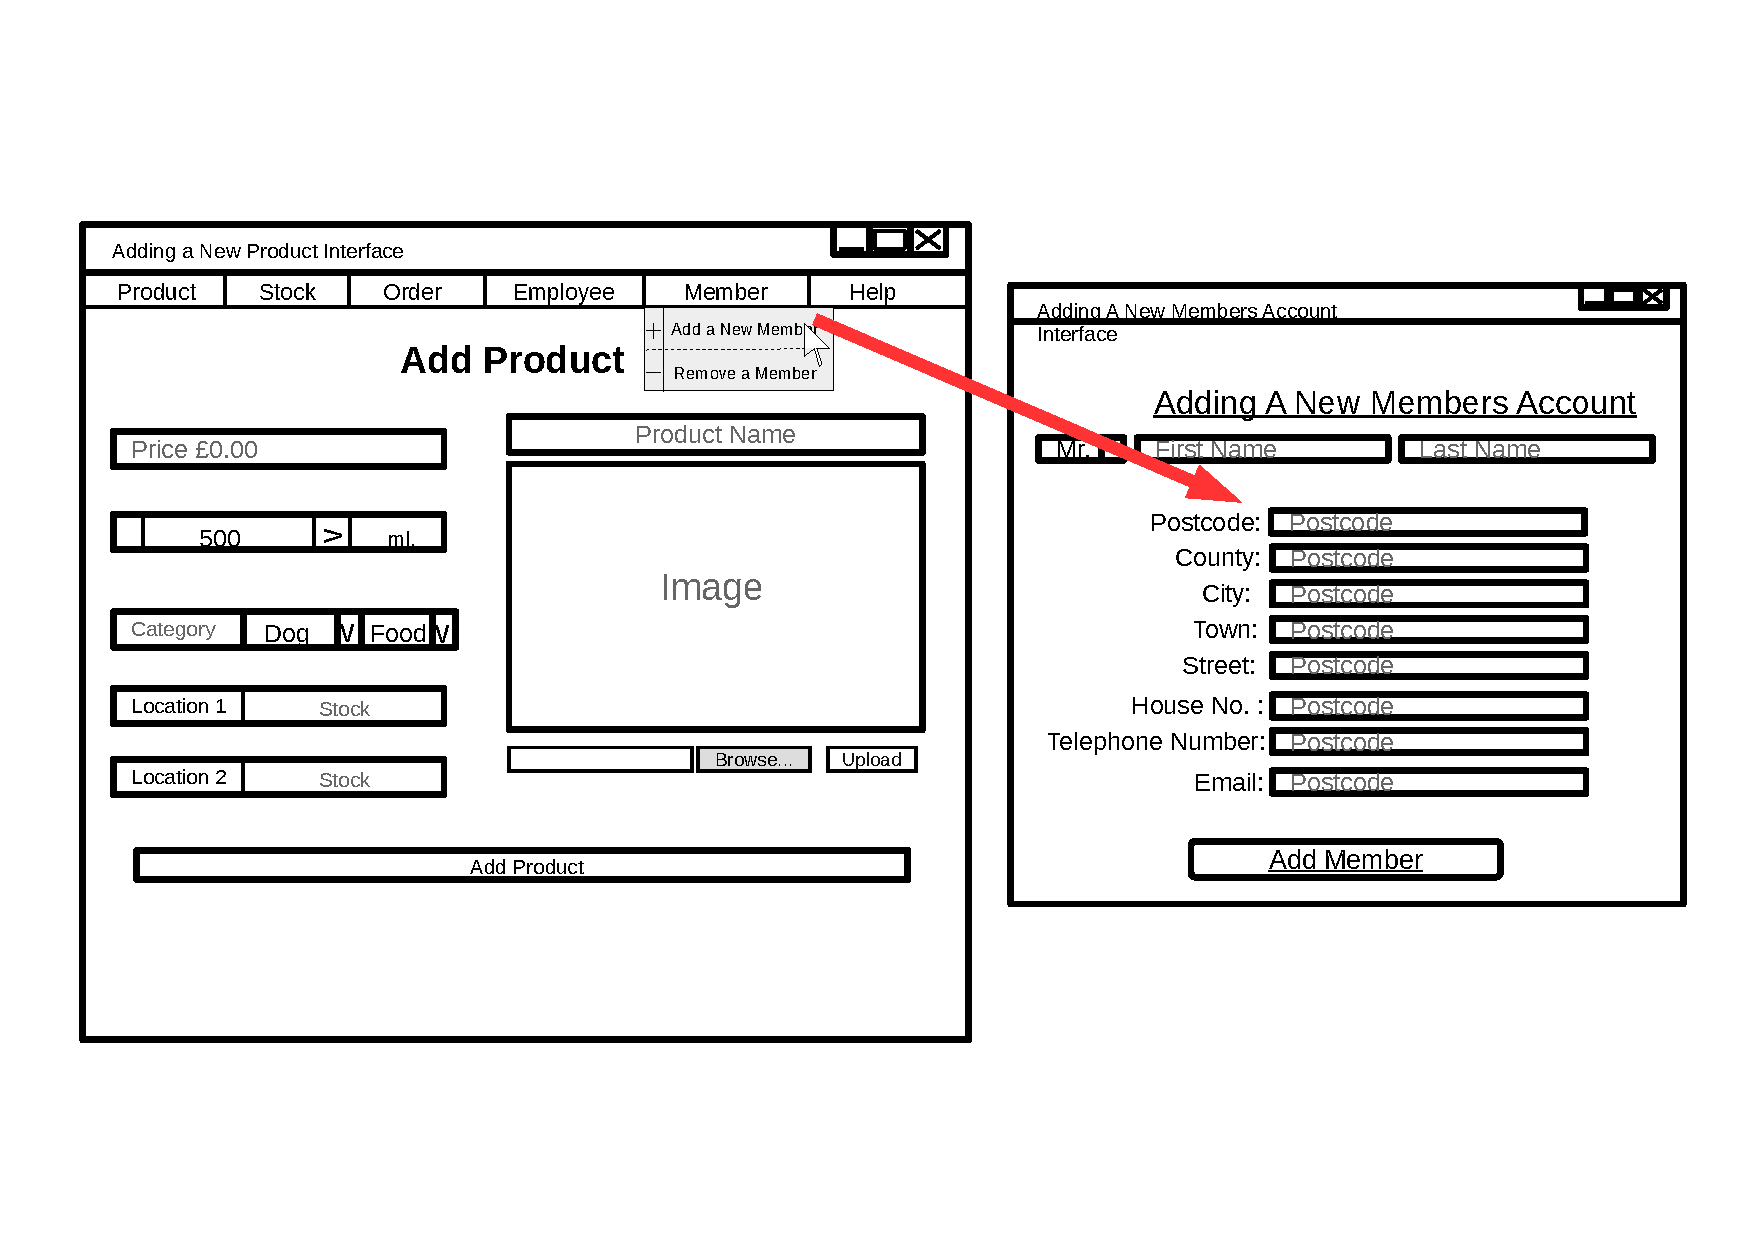
\includegraphics[width = 6cm]{ChangingInterfaceDiagram.pdf}\hspace*{\fill}
\end{figure}

\pagebreak

\begin{figure}[H]
\caption{Adding a New Product} \label{fig:Adding a New Product Interface}
\hfill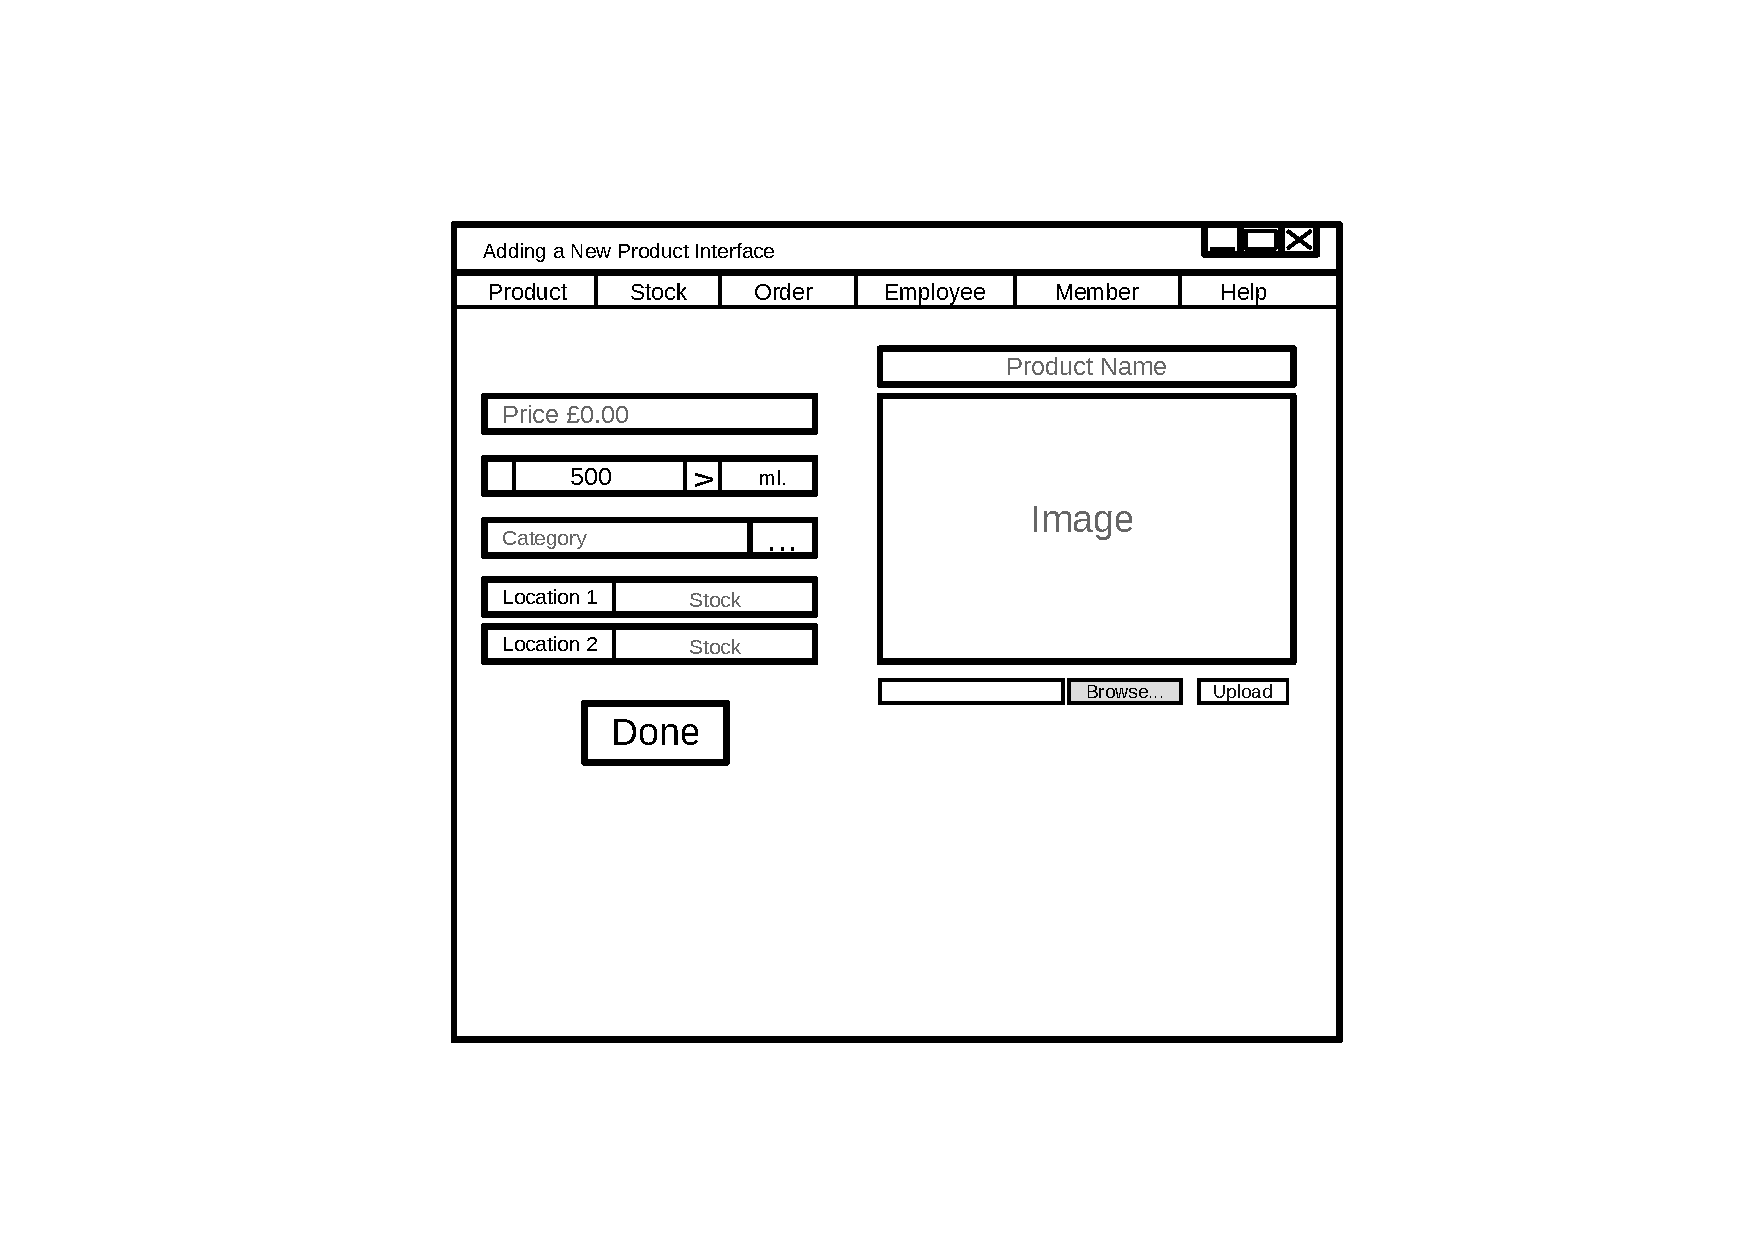
\includegraphics[width = 14cm]{UIDAddingAProductEdited.pdf}\hspace*{\fill}
\end{figure}

Figure 2.15, is the Adding a New Product Interface. Here there is a field in which the user can enter the Product name and the price. To upload an image, the user much click the browse button which will open a window in which the user can select the image file of their choice. once the user has selected the file they must click upload. Once clicked, the upload button will crop the imagine to fit the image area and will display the image to the user, so they can change the image if need be before the product is added to the system. \par

The user has the option to enter any value between 1-1000 in Size field.  This field is to specify the specific size of an item. For example there might be two types of the same dog food, one 500 grams one 750 grams. The value is then followed by a drop down menu. To prevent erroneous data being entered. \par


\begin{figure}[H]
\caption{Drop Down Menu} \label{fig:Drop Down Menu}
\hfill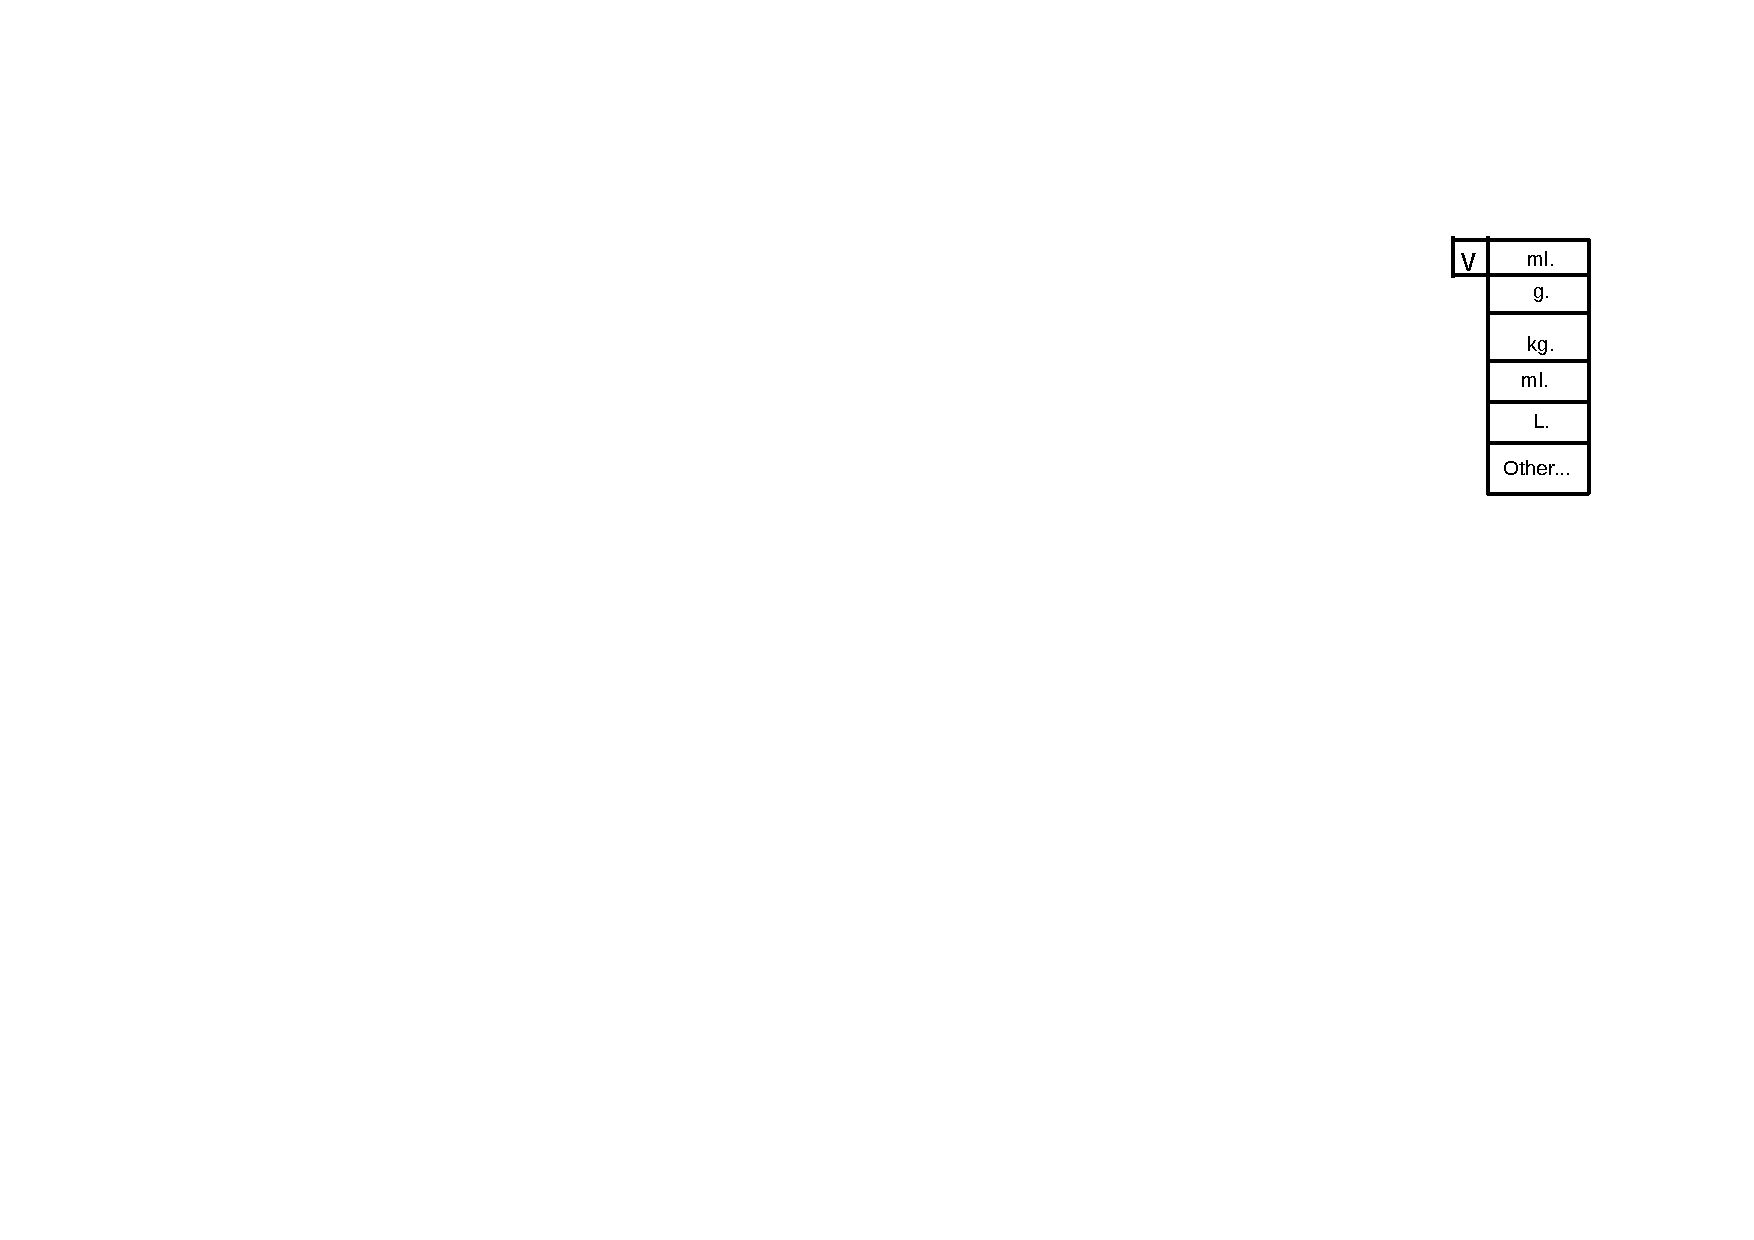
\includegraphics[width = 4cm]{DropDownMenuAddingProduct.pdf}\hspace*{\fill}
\end{figure}

This drop down menu contains the four most common quantities but incase the product does do not fall under any of those quantities, the user can click on the other option, which will allow the user to then enter a custom quantity. \par

The user then has to enter the stock of the product in each location. Once the user has completed all the fields, they can review the information and then click the `Done' button. The `Done' button will then create a New product, with the attributes entered by the user. \par

\begin{figure}[H]
\caption{Adding a New Employee} \label{fig:Adding a New Employee Interface}
\hfill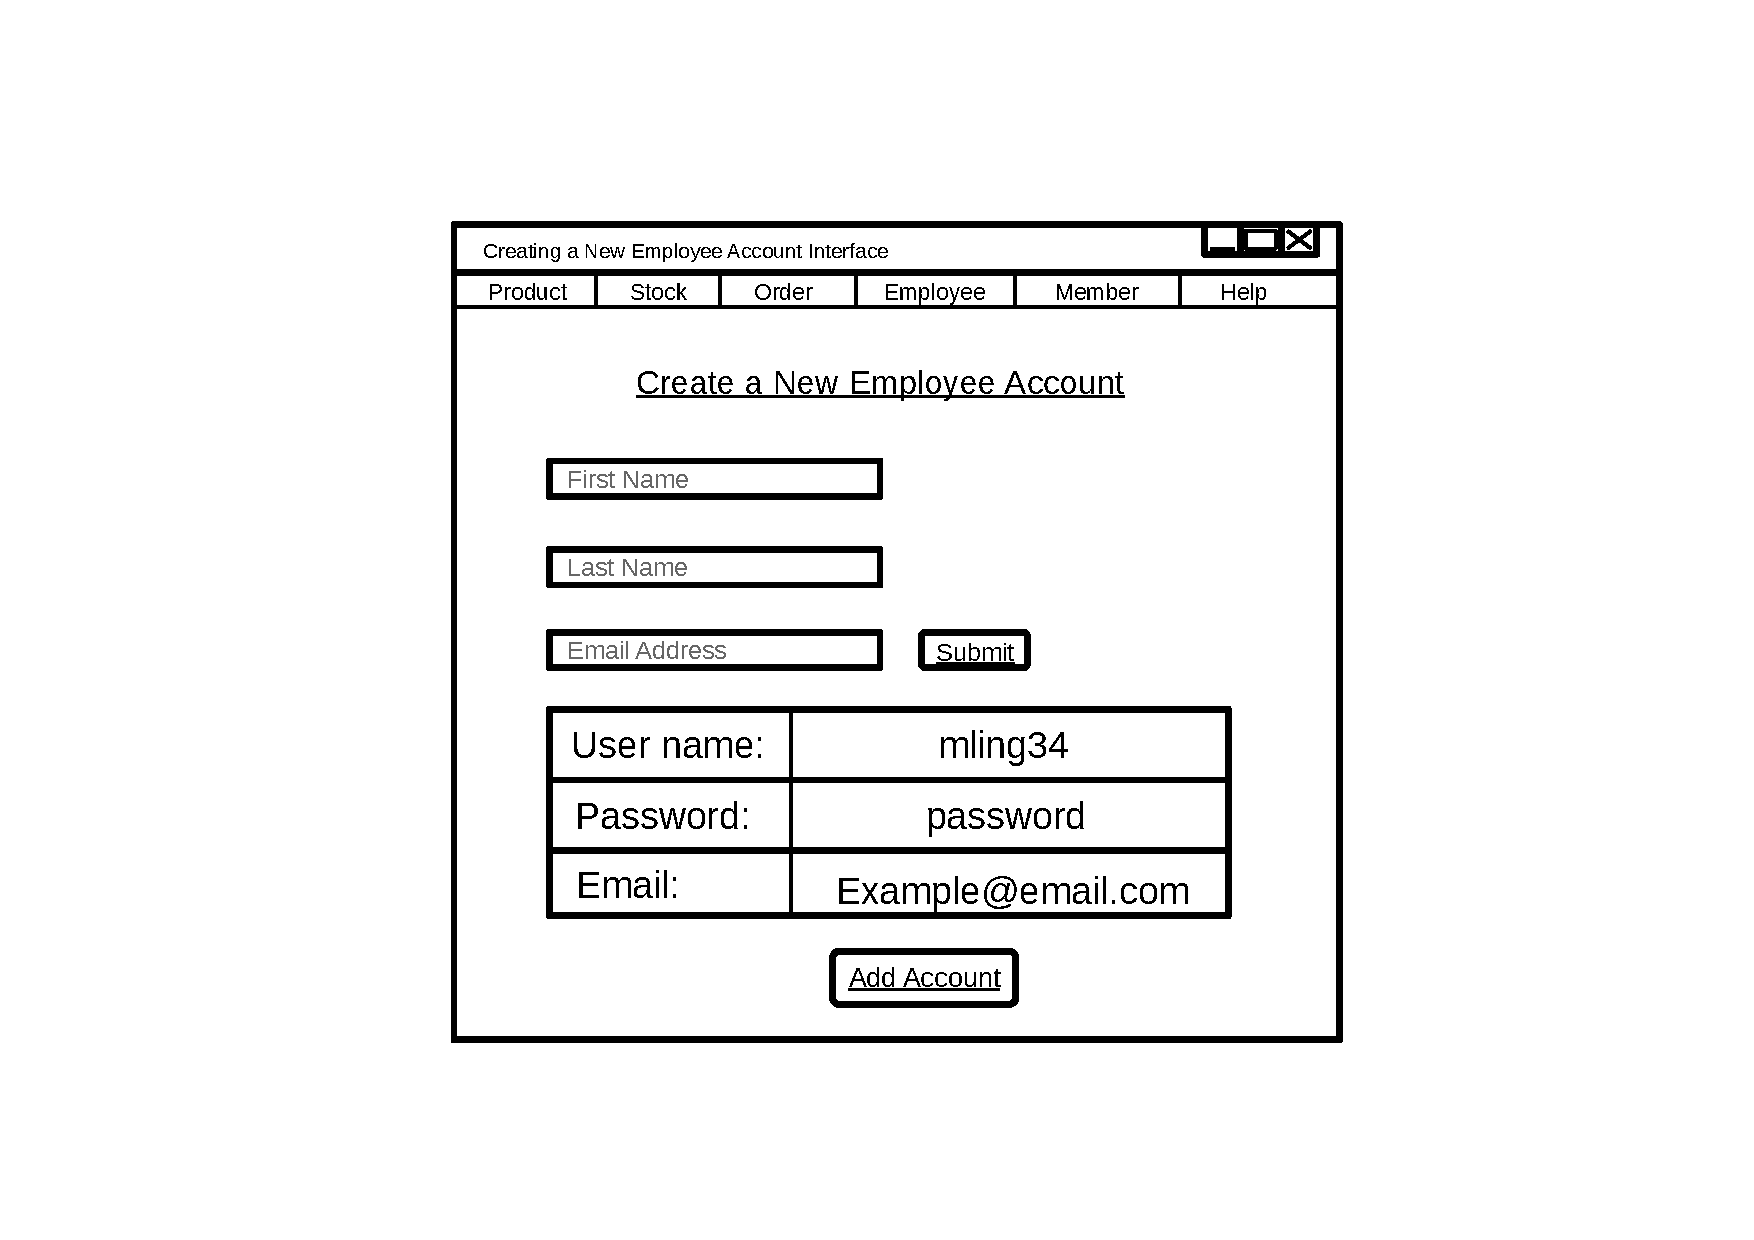
\includegraphics[width = 14cm]{CreatinganEmployeeAccountDiagramEdited.pdf}\hspace*{\fill}
\end{figure}

The `Creating a New Employee Account' interface is very basic. It contains three fields in which the user enters the first name, last name and email address. Once the user has entered the details they can click the `Submit' button. Clicking the `Submit' button will the display the information in the table which will allow the user the review the information they have entered and make changes where necessary. Once the user has entered the correct information they can click the `Add Account' button. This button will then add a new employee to the system with the attributes entered by the user. The new Employee account can then be used when logging in, the new employee can simply enter the password 'Password', where they will then be taken to a screen to change their password tto something more secure. \par

For security, this interface should only be accessible by my client (the administrator) so employees cannot create and delete other employees. If an Employee that is not an administrator is logged on, the option for add Employee and delete Employee should be grayed out and an appropriate message should be displayed in the drop down menu, telling the user why they cannot access this area of the system. \par

\begin{figure}[H]
\caption{Adding a New Member} \label{fig:Adding a New Member Interface}
\hfill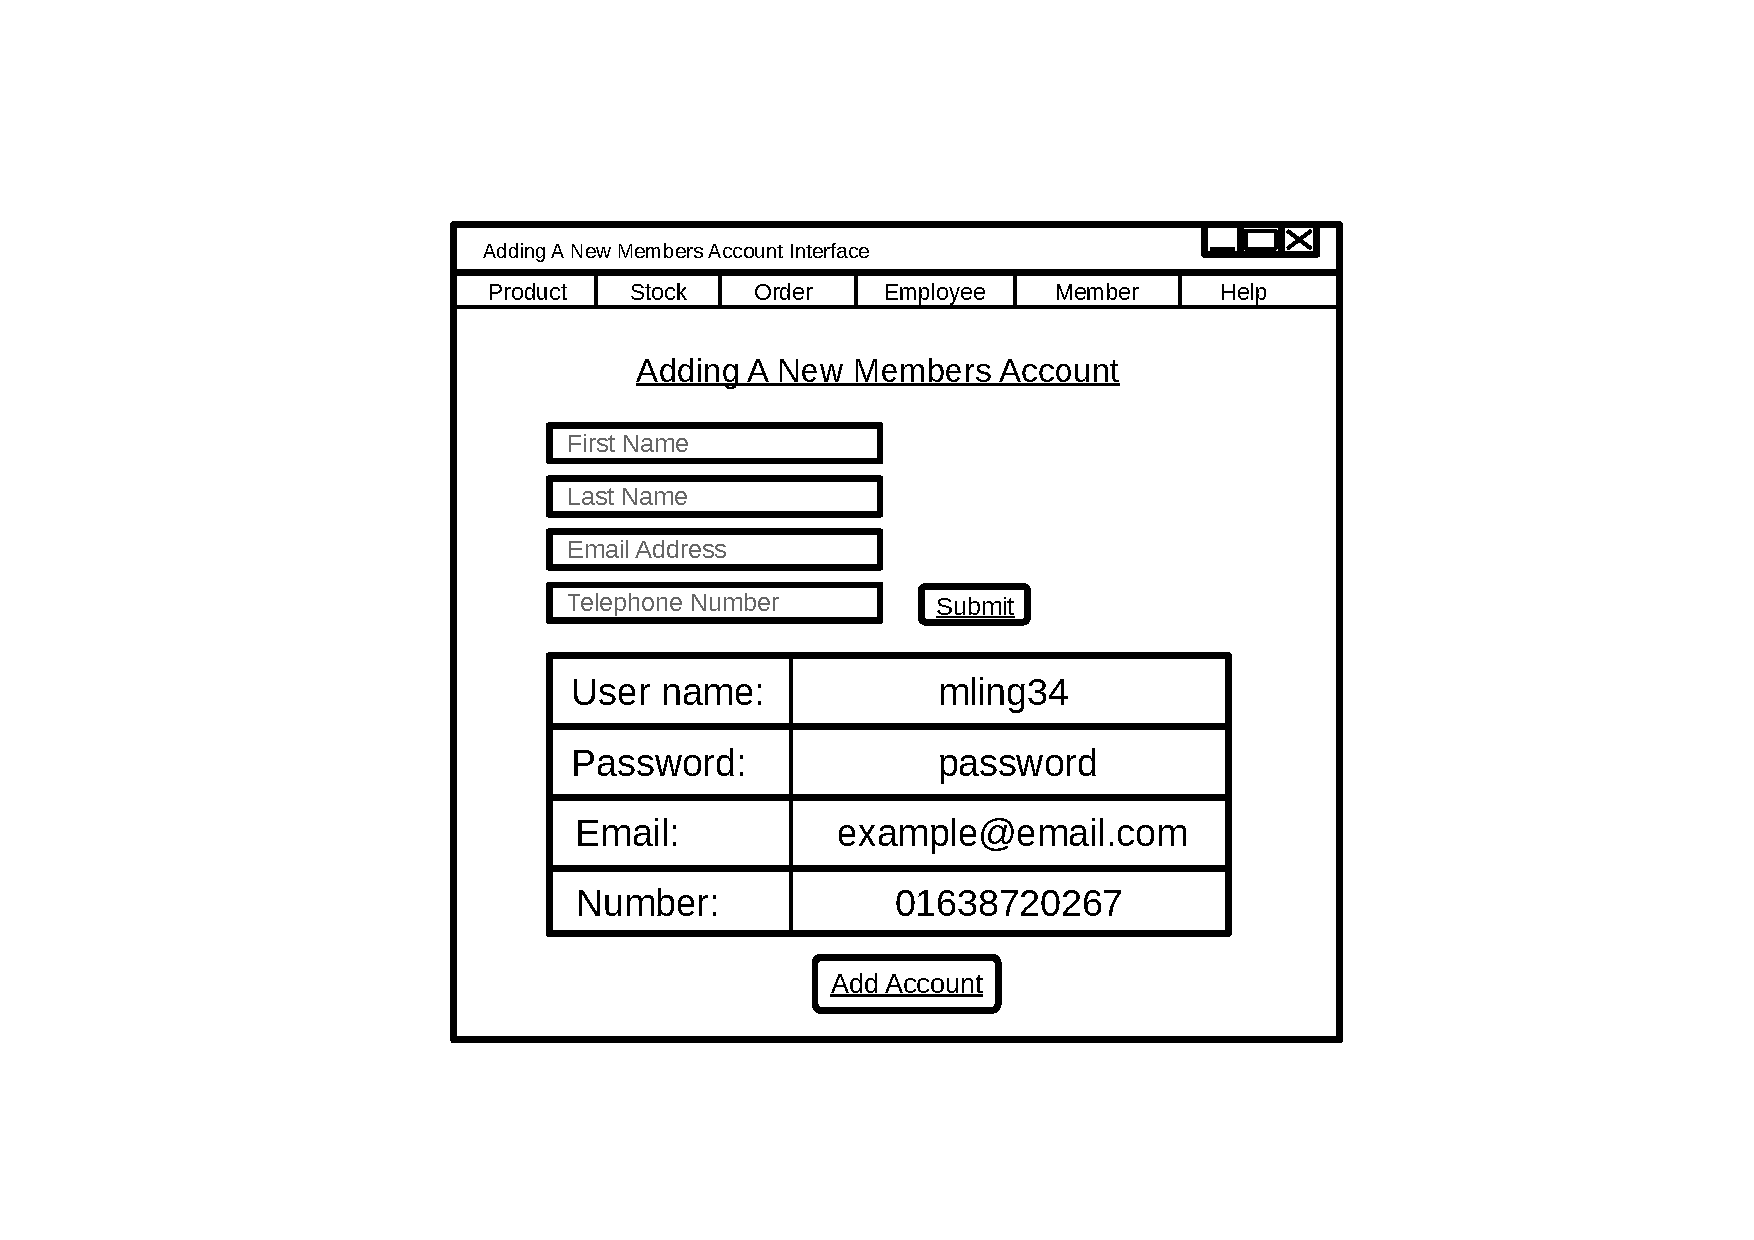
\includegraphics[width = 14cm]{CreatingaMemberDiagramEdited.pdf}\hspace*{\fill}
\end{figure}

Adding a new Member requires the user to enter the most information, mening that creating a new member will take the longesta mount of time. To try and reduce the amount of time entering data i would like to implement the ability to enter the postcode and the rest of the location fields (i.e Street, Town ect..) to be filled out automatically. Once the `Add Account' button is pressed the data entered is added to the database under the Member table. Most, if not all of the  interfaces will have a large underlined title at the top of the interface. This is to prevent the user from entering the wrong details into the wrong interface. For example the user might accidentally enter a Members information into an Employee Account. The title at the top of each interface is to prevent the user from choosing the wrong interface. \par

\begin{figure}[H]
\caption{Stock Management Interface} \label{fig:Stock Management Interface}
\hfill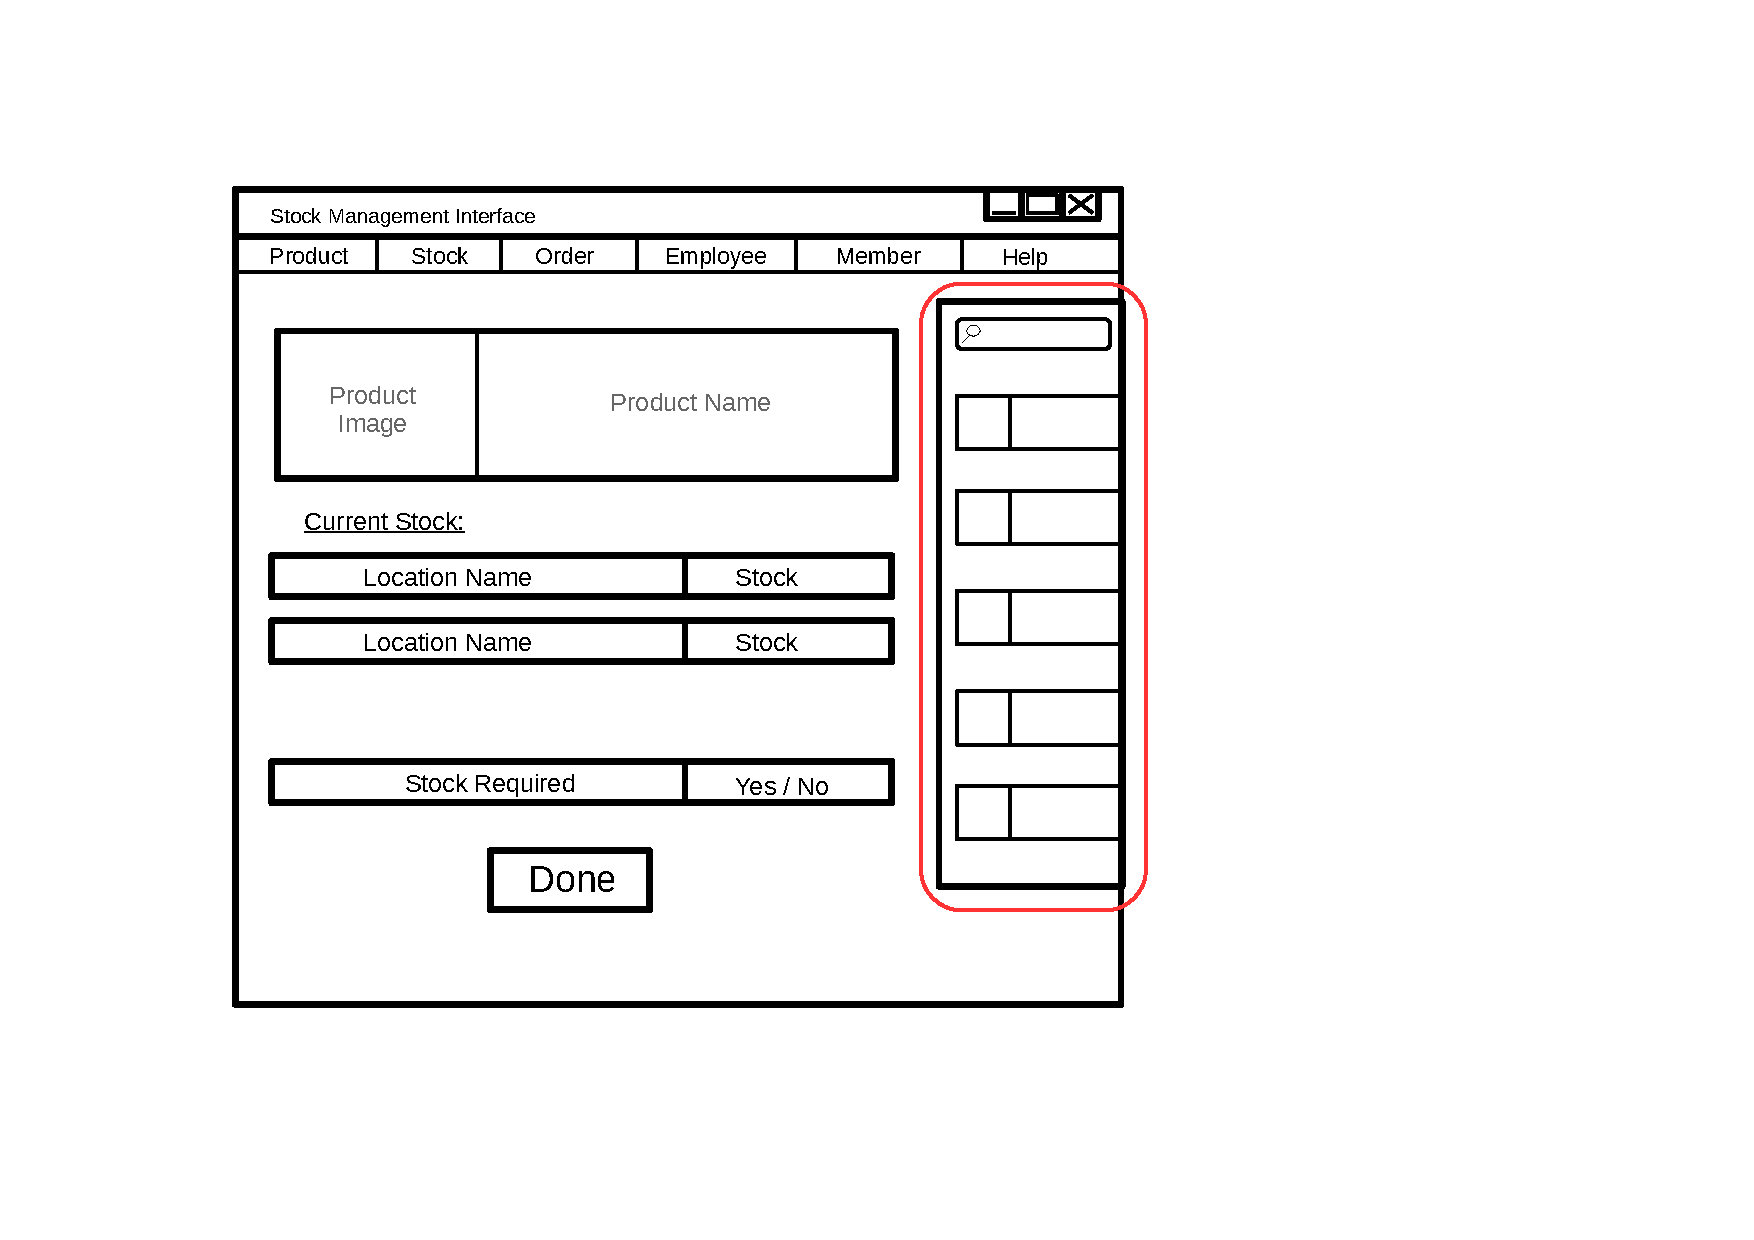
\includegraphics[width = 14cm]{StockManagementDiagramEdited.pdf}\hspace*{\fill}
\end{figure}

Figure 2.19 shows both the Stock Management Interface, but also the search bar. The search bar is circled in red in Figure 2.19, and can be accessed from any of the interfaces other than the log in interface. The search bar allows the User to search for a Product, Employee or Member by entering a string of characters that matches inforamtion stored in the database. for example, entering `food' into the search bar will return any Product with the term `food' in it. \par

  When a match / multiple matches have been found to what is entered into the search field, An image of the product is displayed along with the product name. If the results contain a member or an employee, no image is displalyed just the First and Last name of the member / employee. This sidebar will be accessed using a keyboard shortcut for ease of access and speed of use. \par


\begin{figure}[H]
\caption{Stock Management Interface} \label{fig:Stock Management Interface}
\hfill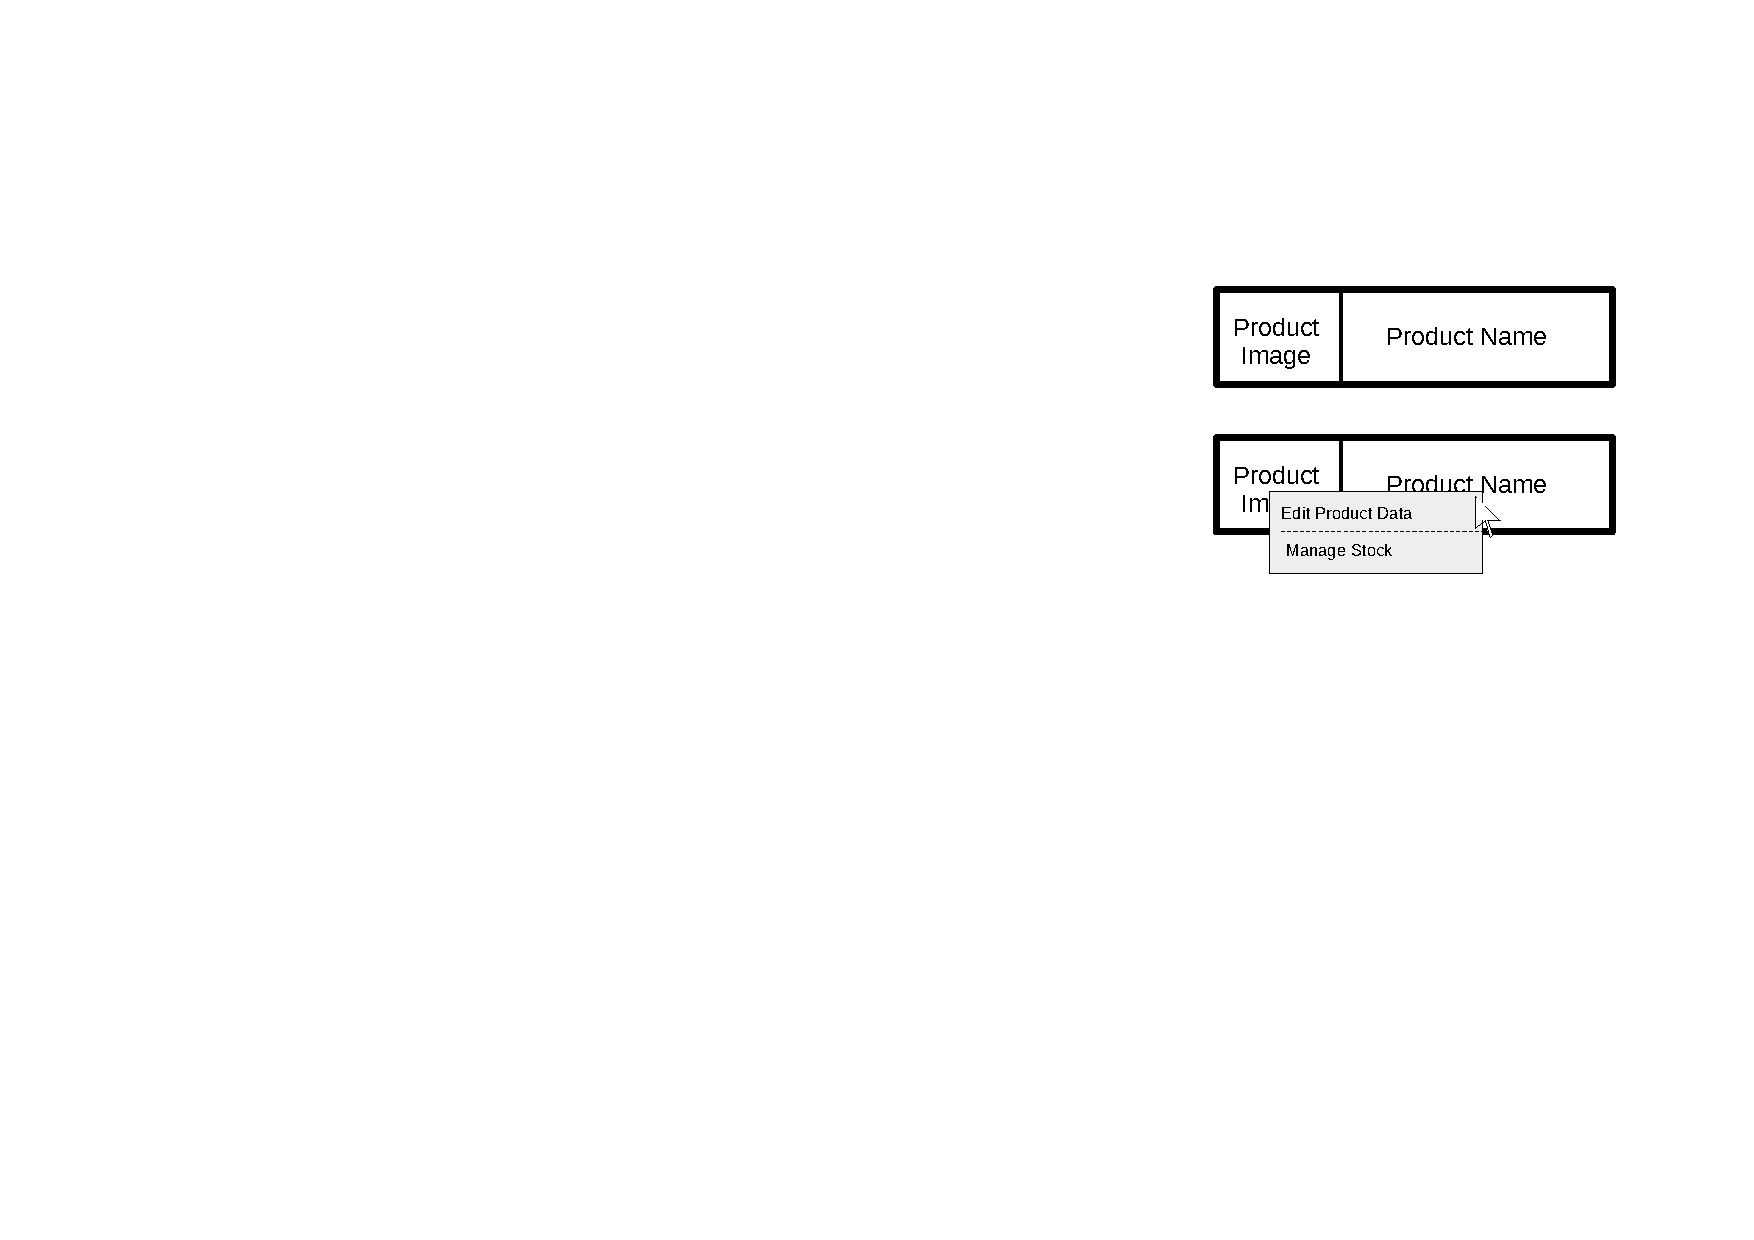
\includegraphics[width = 7cm]{StockManagementDiagramRightClick.pdf}\hspace*{\fill}
\end{figure}

Once the user finds the product they were looking for, they can right click the Product Name or the image and a drop down menu will appear. The user can then either Edit the Product Data or Manage the stock of that specific product. The information about a member is not liekly to change often, but is still possible, therefore, when the user right clicks on the member returned from the search, a similar drop down menu will be displayed and the user will be able to edit the Members details. \par

Going back to Figure 2.19. The stock Management Interface displays the image and name of a product and wil also display the current stock in each location and a will display a boolean variable if more stock of that product is required. The user can change the stock in each location by double clicking the current stock, which will allow the user to delete the old stock and enter the new stock. Once the user has edited the stock they can hit the `Done' button which will return them to the Product Search Interface.\par

The user will not be able to change the products image or name here. This can be done by going to the Product tab and selecting Edit Product. This will take the User to the `Edit Product Interface, where the user can either enter the ProductID of the product they want to edit. If the user does not know the productID of the product they want to edit, the user can go to the product search interface, by going to the Product Menu, then Find a Product. Here the user will be able to search for the product and find its ProductID. I would also like the implement the ability for the user to right click a Product within the Find Product Interface and have the option to Edit Product Data from here. They will then automatically be taken to the edit Product interface, the Product ID field will allready be filled in and the current product information will be displayed to the user for them to edit. The user can then change the attributes they want and save the Product with the changed data. 


#############################################

\begin{algorithm}[H]
\label{fig:repeat_pseudo_example}
\caption{Creating A Sales Graph.}
\begin{algorithmic}[1]
import pg
\Function {Creating Graph}{}
\SET {SalesList}{[]}
\SET{SalesWeek1}{CurentDate{Day - 21}}
SalesList.insert{SalesWeek1}
\SET{SalesWeek2}{CurrentDate{Day - 14}}
SalesList.insert{SalesWeek2}
\SET{SalesWeek3}{CurrentDate{Day - 7}}
SalesList.insert{SalesWeek3}
\SET{SalesWeek4}{CurrentDate}
SalesList.insert{SalesWeek4}
\SET {Graph}{pg.GraphicsWindow}
\SET {WeekNo}{1}
\FOR week in SalesList:
	Graph.addPlot(sales, 0 ,WeekNo)
	\SET{WeekNo}{WeekNo + 1}
\EndFor
\EndFunction
\end{algorithmic}
\end{algorithm}

##############################################

\subsection{Explanation of how data output items are generated}

  \begin{tabular}{|p{4cm}|p{4cm}|}
        \hline
	\textbf{Output} & \textbf{ How the Output is Generated}\\ \hline
	{ Deleting or Editing Member} & {The User enters the MemberID of the product they want to Delete or Edit, The System then searches the Member Table in the Database for a matching MemberID. If the MemberID the user entered matches an existing MemberID , the corresponding Member information is output to the User where the information can then be changed.}\\ \hline
	{Deleting or Editing Employee} & {The User enters the EmploeeID of the product they want to Delete or Edit, The System then searches the Employee Table in the Database for a matching EmployeeID. If the EmployeeID the user entered matches an existing EmployeeID , the corresponding Employee information is output to the User where the information can then be changed.}\\ \hline
	{Order}&{ In The Order, The Employee who created the order is displayed at the top of the Order Invoice. The Order also contains the Product Name, Price, Size and Quantity of each product that the Customer purchased. The Total price and discount is also displayed on the Order Invoice.}
	{Search Result}&{When using the Product Search interface, the Employee can enter specific information about a product and any Product that matches the search field will be output to the user. Here the user can choose to edit the product information or search for a different product.Every time the Employee changes the text in the search field, The system searches the Product Table within the database for any matching data with the search. If a match is found all corresponding data about that Product is output to the user.}
	{ProductSearch Pop Up Window} & {Here, the user can search for any information within the database, a Product, a Member or an Employee. The user must know whether they are looking for a Member, Employee or Product as the system will ask the user to know which table to search. The system will display a drop down menu for the user with the option of Product, employee or Member. The User can select each of these options and the Table being displayed will change depending on which option from the dropdown menu the user selects. By Default, The Product Table is displayed and All Products are displayed within the table. If the User Chooses The Member Option, The System should change the current table being displayed to the Members Table. Once the Appropriote table is displayed, The user can then Search The table using specific Keywords and if any data matches the keyword, The Table will display the entire Member or EMployee or Product that corresponds to the matching data.}
	\end{tabular}